% !TeX root = ../thuthesis-example.tex

\chapter{驾驶舱简介}

\section{飞行员驾驶舱}

\begin{figure}[h]
  \center
  \includegraphics[width=0.8\textwidth]{pilotcockpit.png}
\end{figure}

\subsection{左侧控制台}

\subsubsection{抗荷服充气检测按钮}
\begin{figure}[h]
  \center
  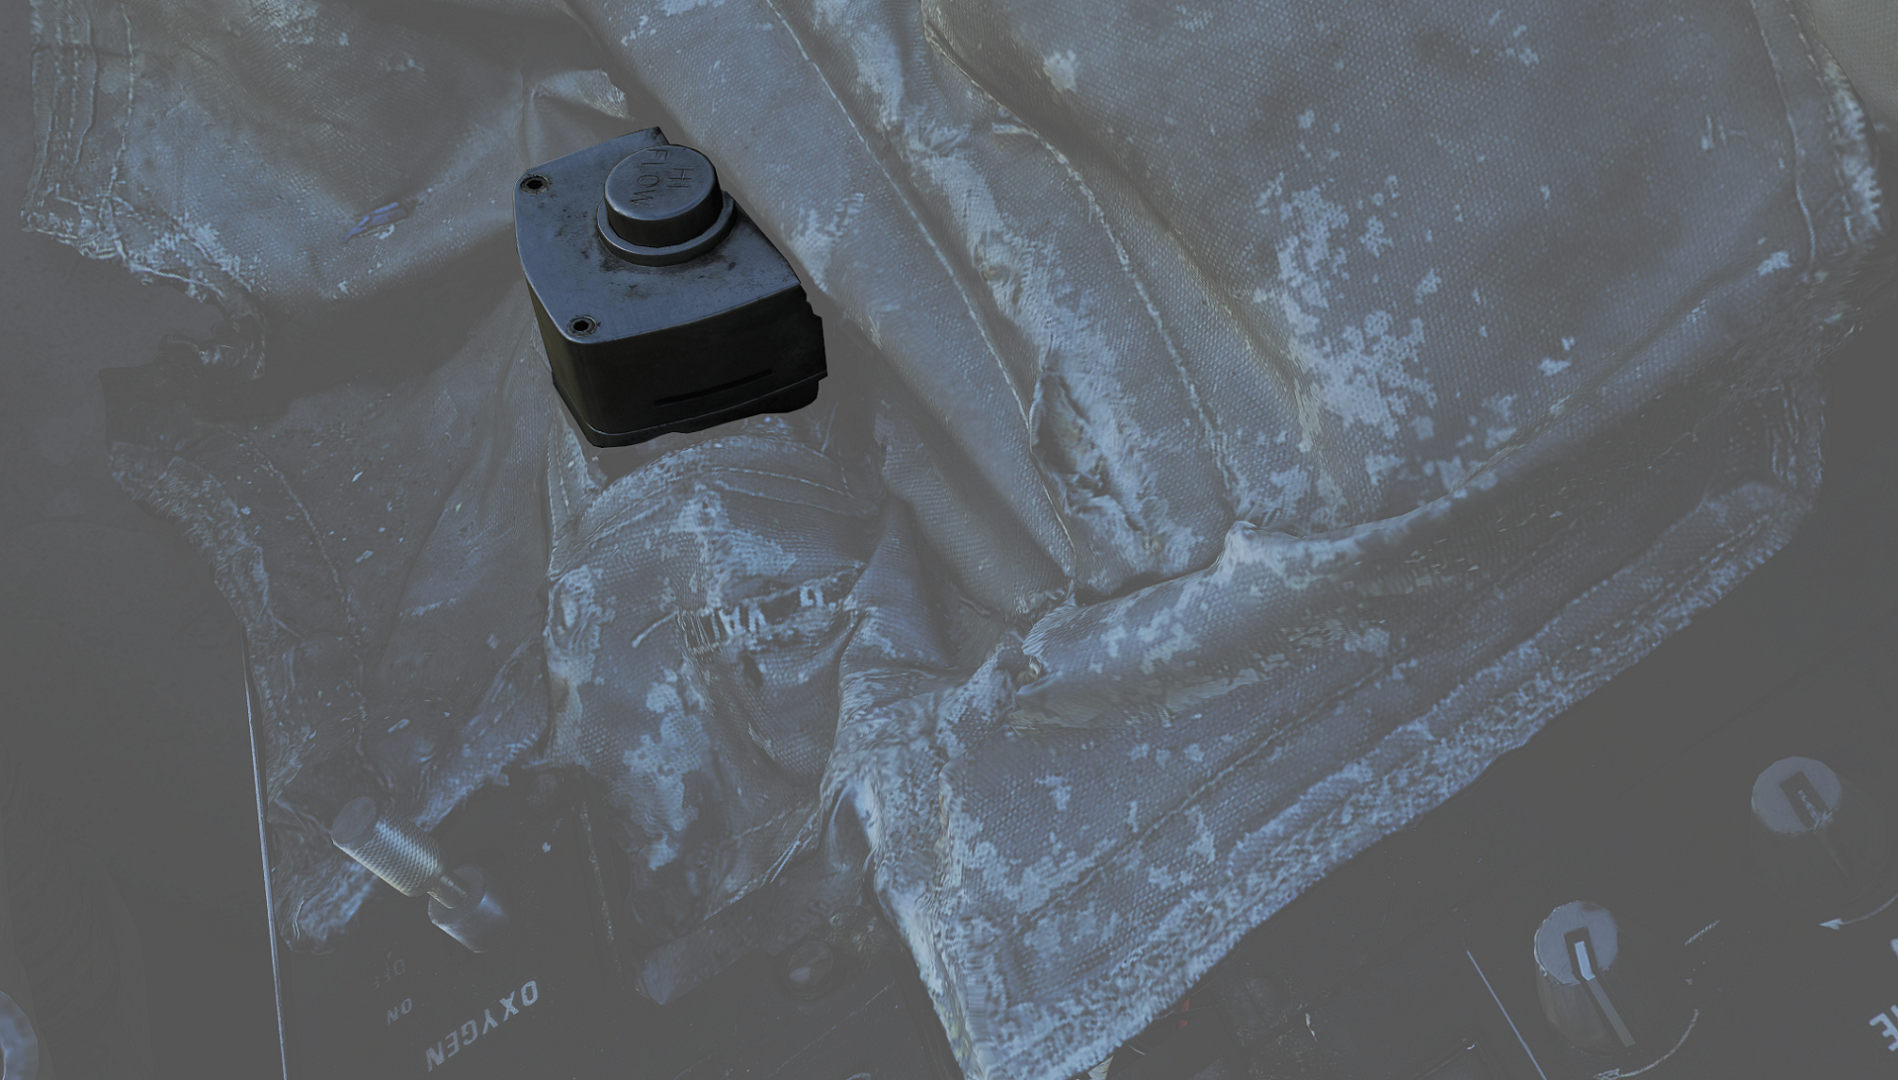
\includegraphics[width=0.8\textwidth]{g-valve.png}
\end{figure}
按下按钮来测试抗荷服充气。

\subsubsection{供氧-通风控制面板}

\begin{figure}[h]
  \center
  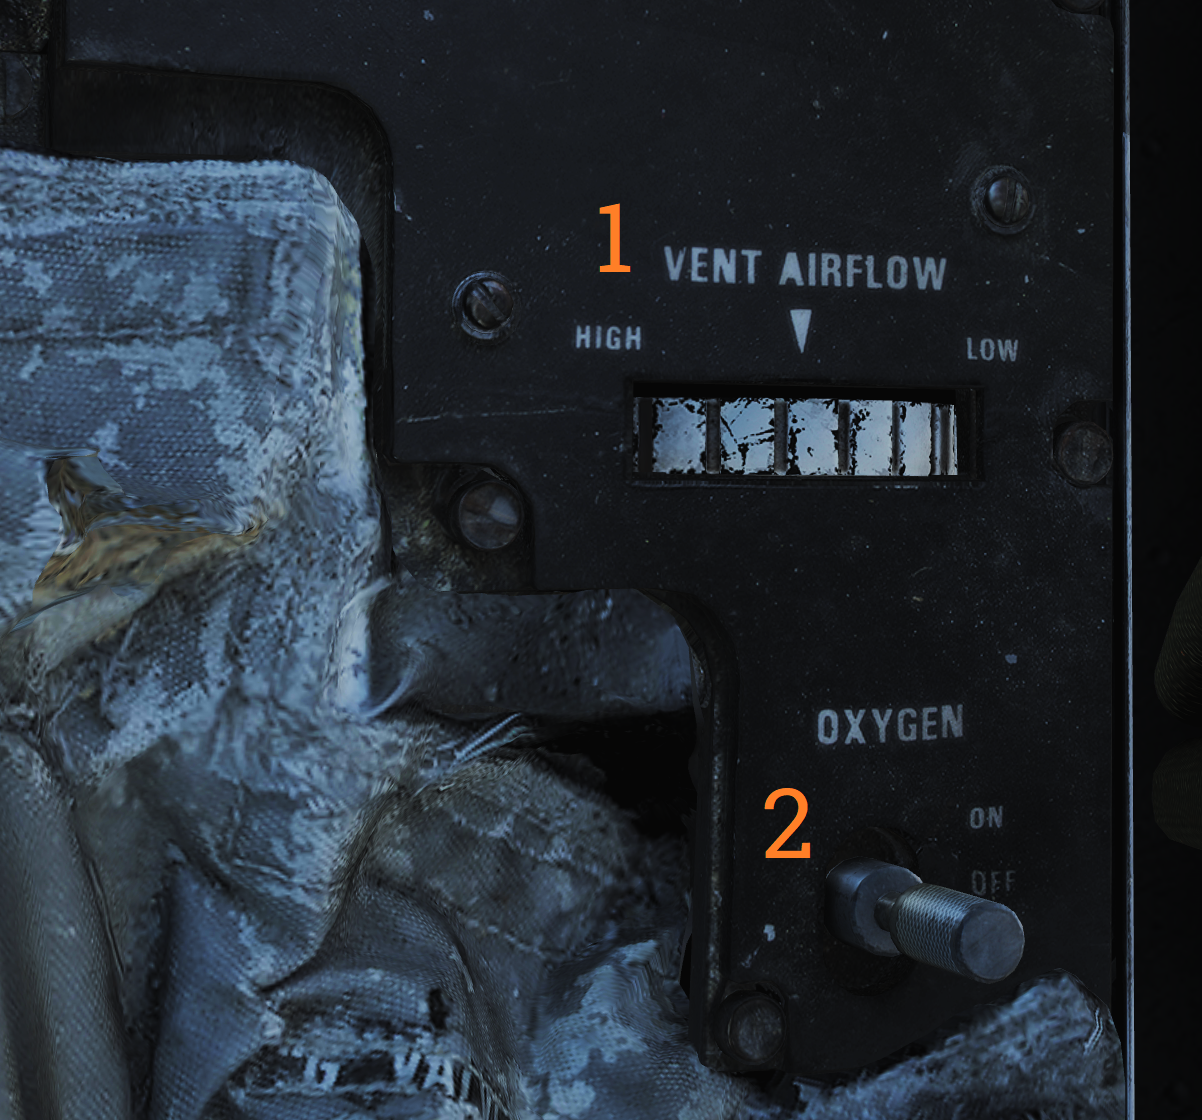
\includegraphics[width=0.8\textwidth]{oxygen-vent.png}
\end{figure}
控制抗荷服或坐垫中的通风气流以及通向飞行员面罩的氧气。

\begin{enumerate}
  \item VENT AIRFLOW 拨轮:通风气流调节拨盘,用于控制抗荷服气流进出,未连接抗荷服时则控制坐垫气流。
  \item OXYGEN 开关::供氧开关,开关有 ON / OFF 两个档位。用于控制流向面罩的氧气。
\end{enumerate}

\subsubsection{音量/TACAN指令面板}

\begin{figure}[h]
  \center
  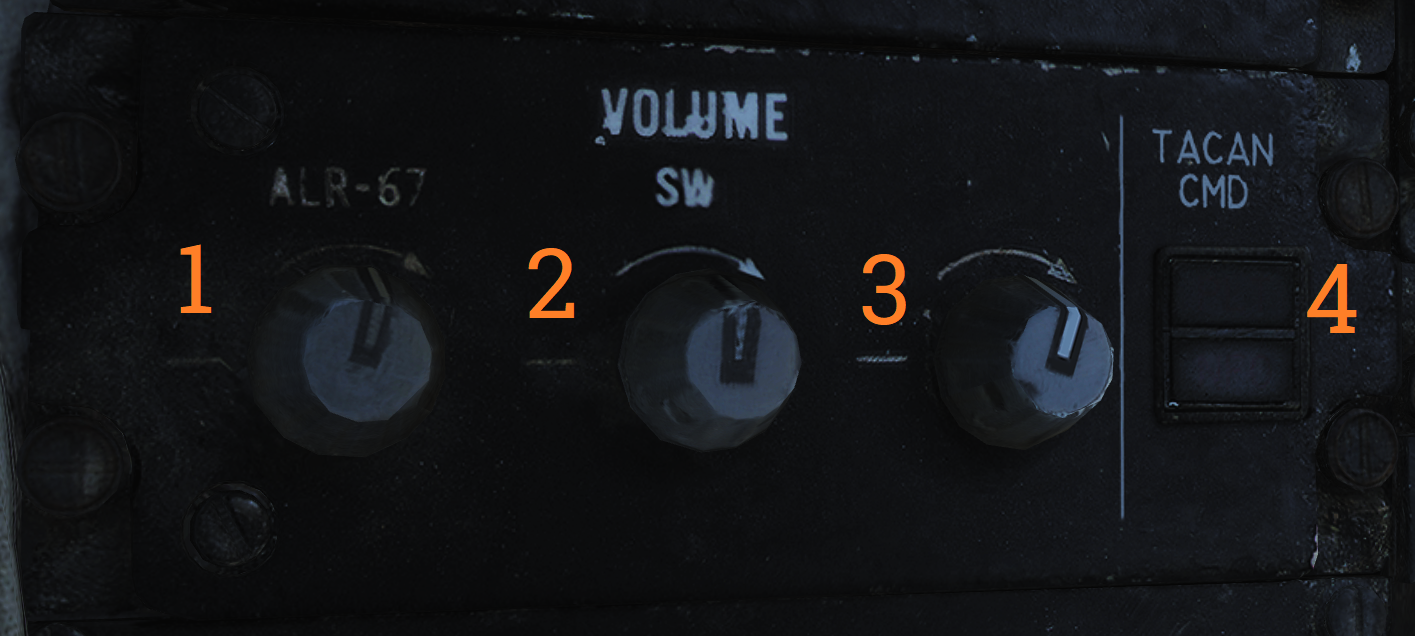
\includegraphics[width=0.8\textwidth]{volume.png}
\end{figure}
用于调整飞行员头戴中的音量和指定控制 TACAN 的乘员。

\begin{enumerate}
  \item ALR-67 旋钮:用于控制飞行员头戴中 ALR-67 的音量。
  \item SW 旋钮:“响尾蛇”音量旋钮,用于调节飞行员头戴中“响尾蛇”导弹的音调音量。
  \item V/UHF 2 旋钮:控制飞行员头戴中 AN/ARC-182 无线电台的音频音量。
  \item TACAN CMD 按钮开关:带有指示灯的按钮开关,用于指定控制 TACAN 设备的乘员(飞行员 / RIO)。指示灯显示当前的设定。
\end{enumerate}

\subsubsection{TACAN控制面板}

\begin{figure}[h]
  \center
  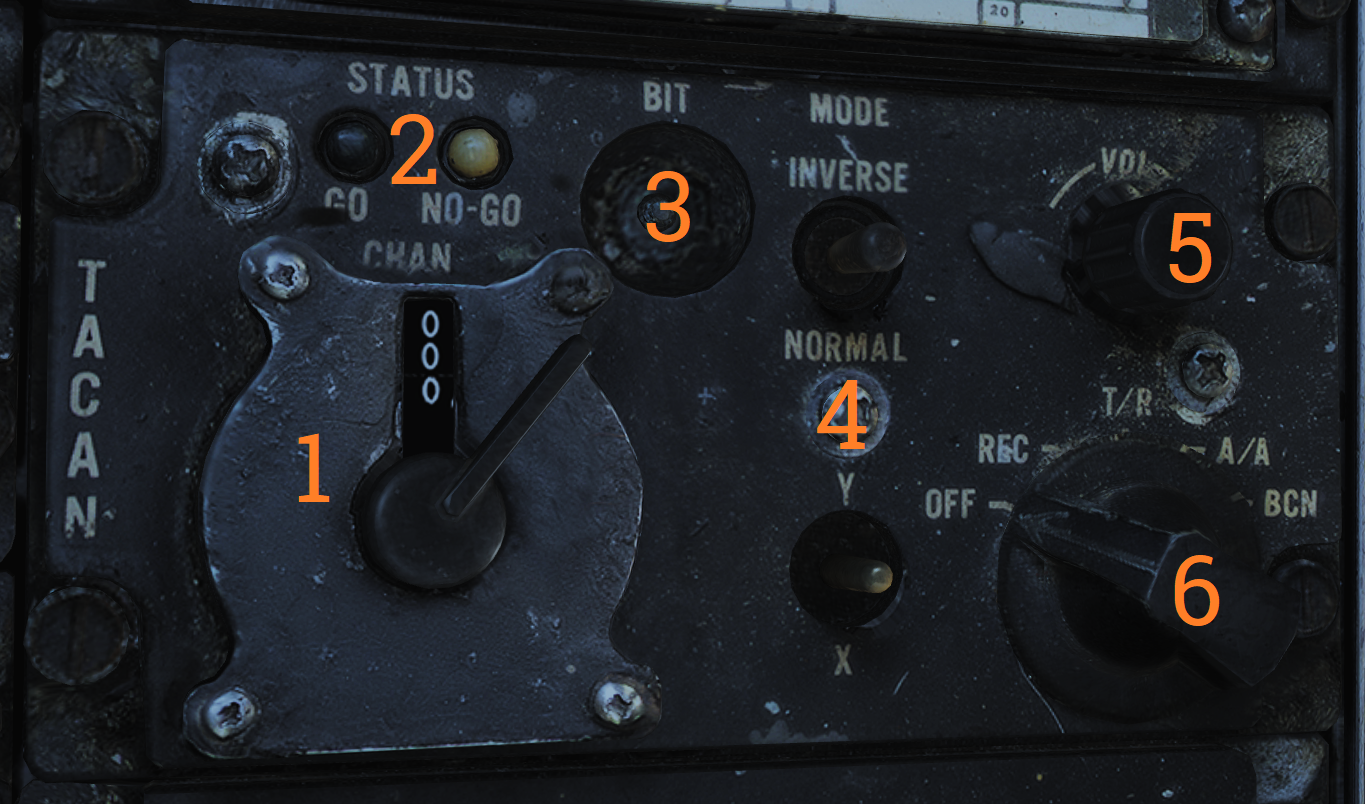
\includegraphics[width=0.8\textwidth]{tacan.png}
\end{figure}
如果飞行员有 TACAN 设备控制权,则可以通过该控制面板操作 TACAN。

\begin{enumerate}
  \item 双层旋转开关:使用外侧拨盘选择 TACAN 波道的前两位数字,使用内侧拨盘选择最后一位数字。
  \item GO 和 NO-GO 灯:通过/未通过指示灯,指示 TACAN 是否通过自检。
  \item BIT 按钮:自检按钮,按下按钮开始 TACAN 自检。
  \item MODE 开关:波段模式选择开关,用于切换 TACAN 工作波段,可以选择 X 或 Y 波段。INVERSE 模式无功能。
  \item VOL 旋钮:音量旋钮,用于调节飞行员 TACAN 音频音量。
  \item 模式选择旋钮:用户选择TACAN工作模式。
  \begin{itemize}
    \item OFF:关闭 TACAN。
    \item REC:仅接收信号。
    \item T/R:传输并接收信号,该模式下TACAN可以进行测距。
    \item A/A:空对空TACAN模式。
    \item BCN:信标TACAN模式(无功能)。
  \end{itemize}
\end{enumerate}

\subsubsection{机内通话系统控制面板}

\begin{figure}[h]
  \center
  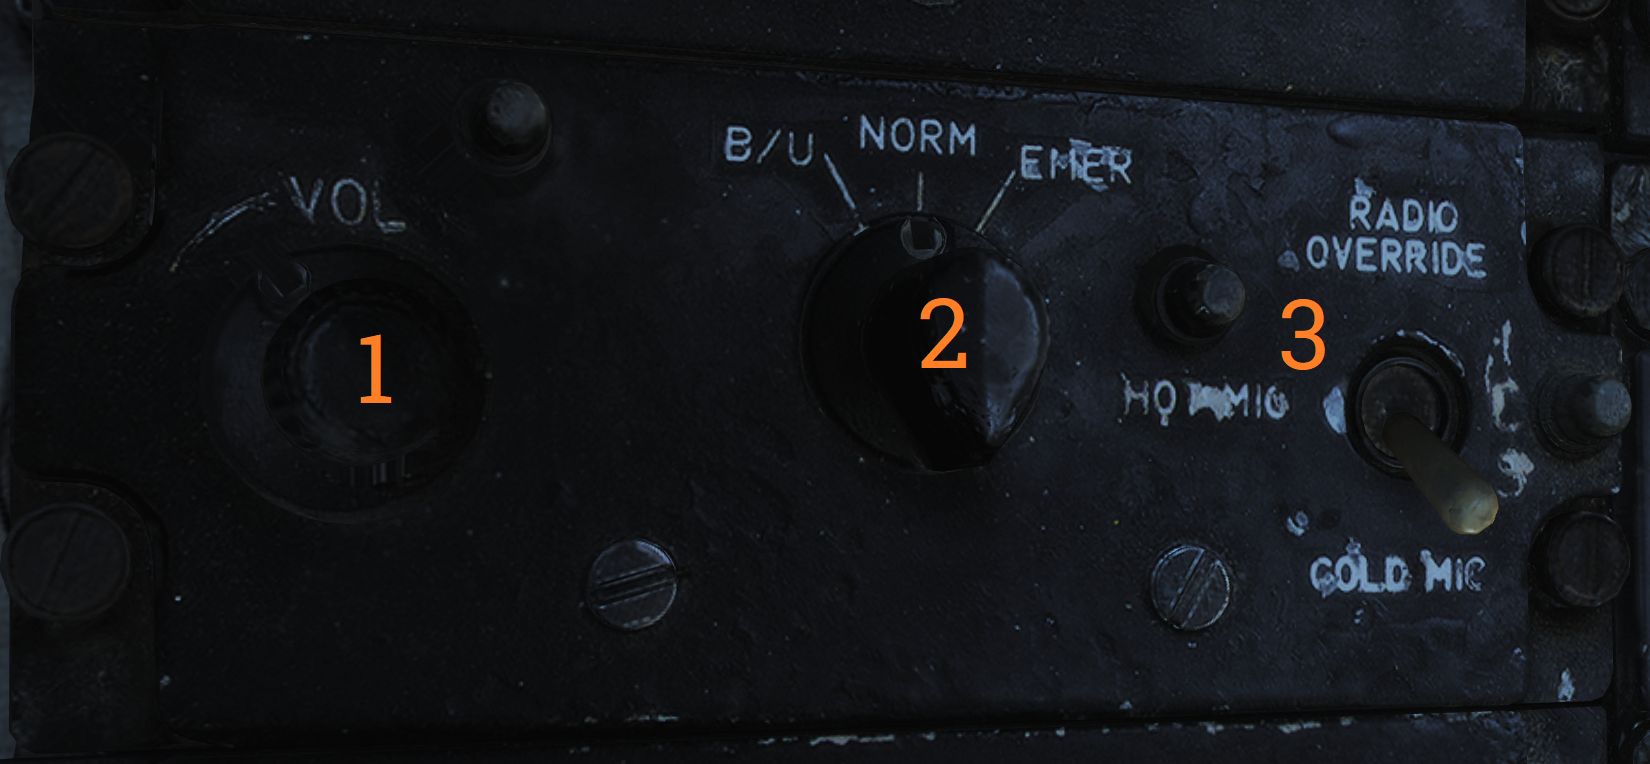
\includegraphics[width=0.8\textwidth]{ics.png}
\end{figure}
用于控制机内通话系统(ICS)。
\begin{enumerate}
  \item VOL旋钮:音量旋钮,用于调节飞行员接收 RIO 对讲音频的音量。
  \item 放大器选择旋钮:用于选择处理飞行员头戴音频的放大器。
  \begin{itemize}
    \item B/U:备用放大器。
    \item NORM:正常放大器。
    \item EMER:应急放大器。这个档位会使用 RIO 的放大器和他的音量设定。启用应急放大器时,飞行员将无法监听只有常规放大器中飞行员才能听见的 “响尾蛇” 导弹音调和发动机失速 / 超温警告音。
  \end{itemize}
  \item ICS控制开关:用于选择 ICS 的功能。
  \begin{itemize}
    \item RADIO OVERRIDE:无线电台超控,让 ICS 音频替换无线电音频。
    \item HOT MIC:RIO 无需按下 PTT(Push-To-Talk,按键通话)开关即可进行对讲。地勤人员也可以通过外部对讲机与乘员通话。
    \item COLD MIC:RIO 需按下 PTT 开关才能对讲。
  \end{itemize}
\end{enumerate}

\subsubsection{AFCS控制面板}

\begin{figure}[h]
  \center
  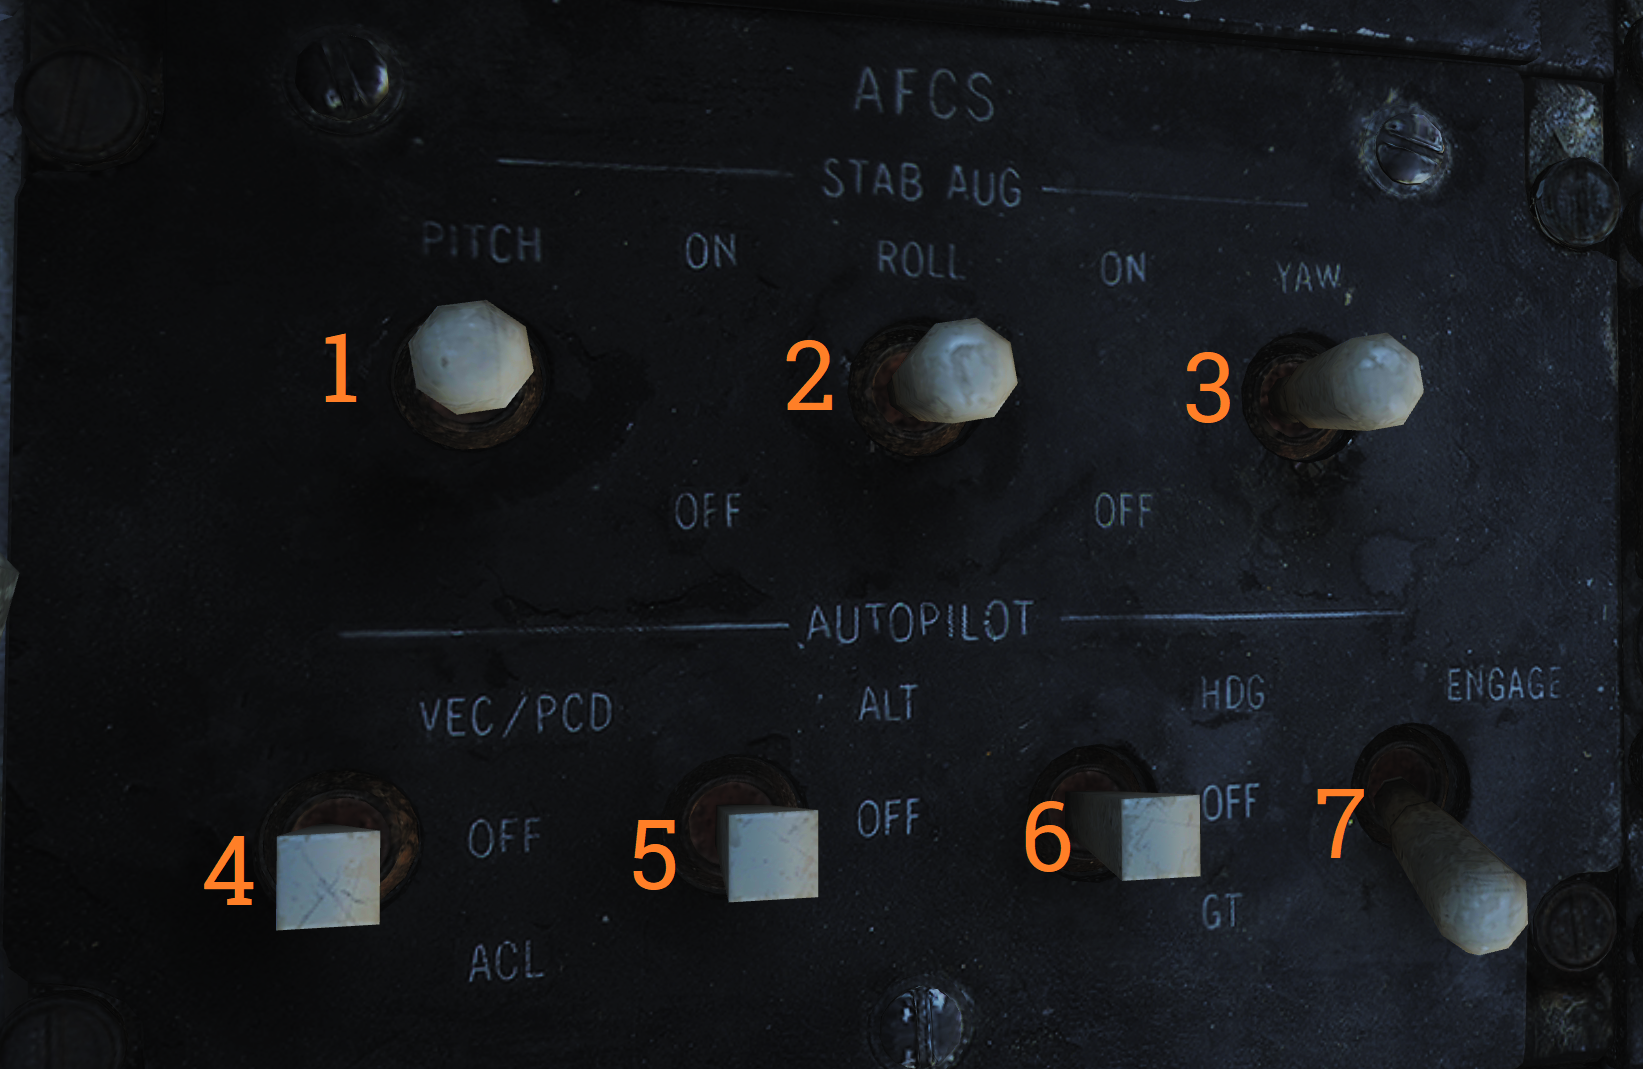
\includegraphics[width=0.8\textwidth]{afcs.png}
\end{figure}
用于控制自动飞控系统(AFCS)和自动驾驶。

\begin{enumerate}
  \item PITCH 开关:启用俯仰通道增稳。
  \item ROLL 开关:启用滚转通道增稳。
  \item YAW 开关:启用偏航通道增稳。
  \item VEC/PCD/ACL 开关:用于切换自动驾驶远程控制模式。
  \begin{itemize}
    \item VEC/PCD:引导航向/精确航线方向模式。数据链路控制飞机滚转和俯仰轴。这个模式通过飞行员驾驶杆上的 NWS(前轮转向)按钮激活。
    \item OFF:功能关闭。
    \item ACL:自动助降模式,这个模式通过飞行员驾驶杆上的 NWS 按钮激活。
  \end{itemize}
  \item ALT开关:高度保持开关,开关有 ALT / OFF 两个档位,用于启用自动驾驶高度保持。这个功能通过飞行员驾驶杆上的 NWS 按钮激活。
  \item HDG开关:航向保持开关,用于选择航向保持模式。
  \begin{itemize}
    \item HDG:启动航向保持模式。
    \item OFF:关闭航向保持模式。
    \item GT:启用地面轨迹模式,通过飞行员驾驶杆上的 NWS 按钮激活。
  \end{itemize}
  \item ENGAGE 开关:自动驾驶控制开关,有 ENGAGE / OFF 两个档位,分别启用和关闭自动驾驶。
\end{enumerate}

\subsubsection{UHF 1(AN/ARC-159)无线电台}

\begin{figure}[h]
  \center
  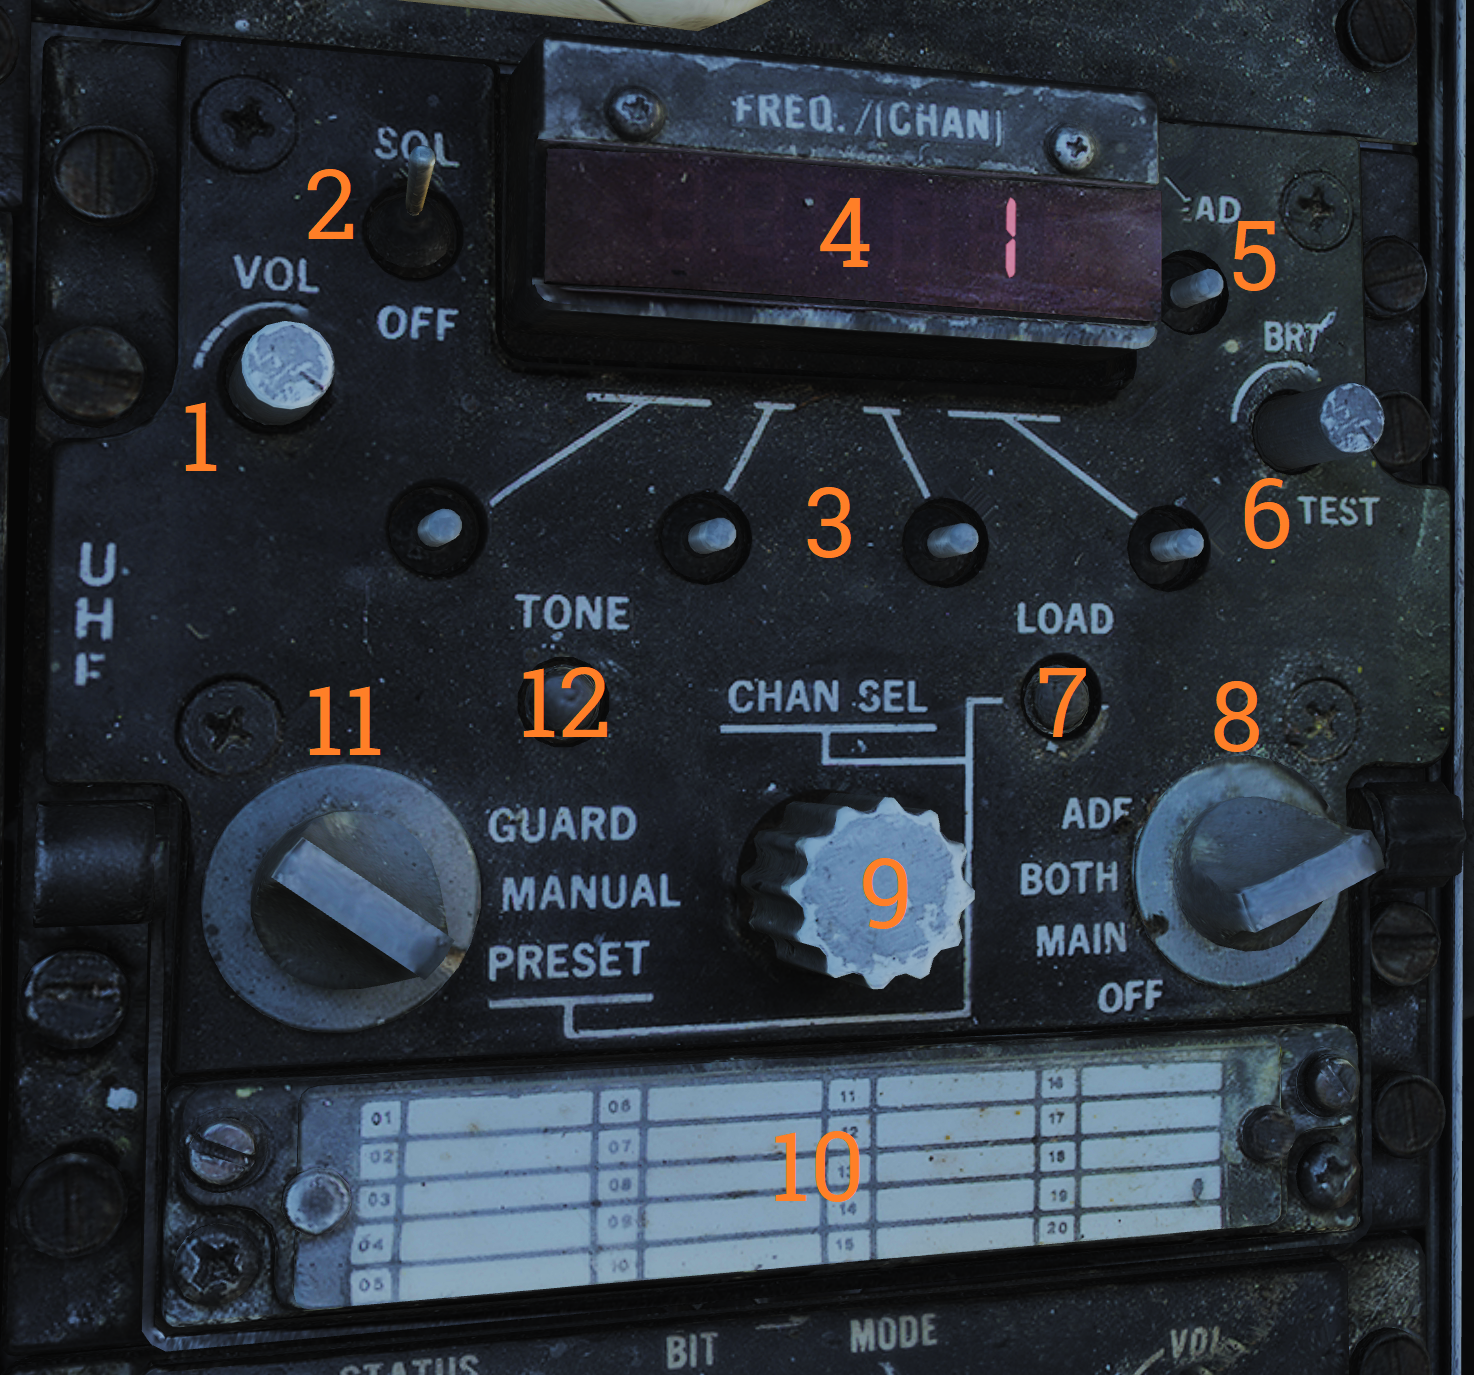
\includegraphics[width=0.8\textwidth]{arc-159.png}
\end{figure}
1号 UHF 电台及其控制组件。

\begin{enumerate}
  \item VOL 旋钮:音量旋钮,用于调节飞行员头戴中的 UHF 1 音频音量。
  \item SQL 开关:静噪控制开关,有 ON / OFF 两个档位,分别用于开启或关闭静噪。
  \item 频率选择开关:频率选择拨动开关,用于调定频率。
  \item FREQ./(CHAN) 显示窗:频率 /(波道)显示窗,用于显示当前选中的频率或波道。
  \item READ开关:读取控制开关,按住开关时,频率/(波道)显示窗将显示预设波道的频率。
  \item BRT旋钮:亮度旋钮,用于调节显示屏的亮度。
  \item LOAD按钮:加载按钮,用于加载预设波道的显示频率。
  \item 功能选择旋钮:用于选择无线电功能,该旋钮的四个档位分别是 ADF、BOTH、MAIN 和 OFF。
  \item CHAN SEL旋钮:波道选择旋钮,用于选择预设波道。
  \item 预设波道表:用于记录频率或预设波道的作用。
  \item 模式选择旋钮:这个旋钮用于选择无线电频率模式(GUARD - 救生频率,MANUAL - 手动频率,PRESET - 预设频率)。
  \item TONE按钮:音调按钮,按住按钮会在当前无线电频率上发送一个单音(频率为1,020赫兹)。
\end{enumerate}

注意:AN/ARC-159 中的 ADF 无功能,改为使用 V/UHF 2中的 ADF。

\subsubsection{不对称推力限制器 / 发动机模式选择}

\begin{figure}[h]
  \center
  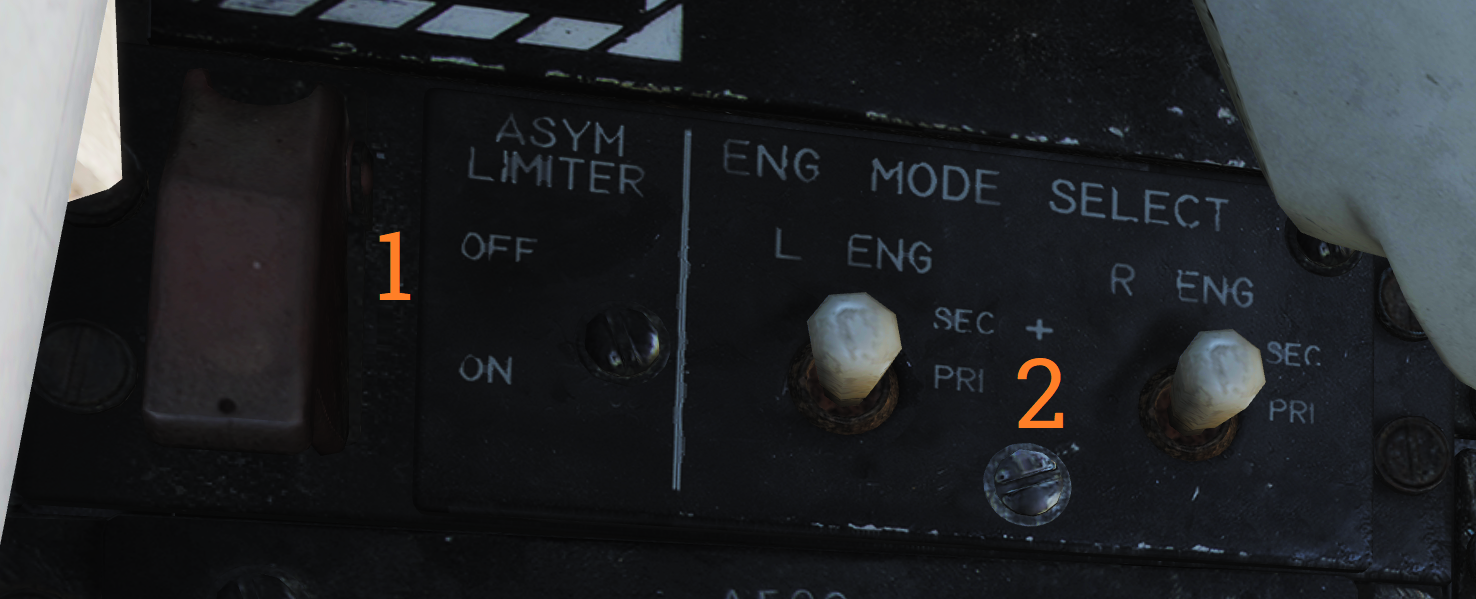
\includegraphics[width=0.8\textwidth]{asym.png}
\end{figure}
这个面板用于控制不对称推力限制系统和发动机控制模式。

\begin{enumerate}
  \item ASYM LIMITER 开关:不对称推力限制器开关,带有保护盖,开关 ON / OFF 两个档位分别启用和禁用不对称加力推力限制器。
  \item ENG MODE SELECT 开关:发动机模式选择开关,用于选择左右发动机各自的控制模式。
  \begin{itemize}
    \item PRI:主要控制模式。
    \item SEC:次要控制模式。
  \end{itemize}
\end{enumerate}

\subsubsection{目标指定开关}

\begin{figure}[h]
  \center
  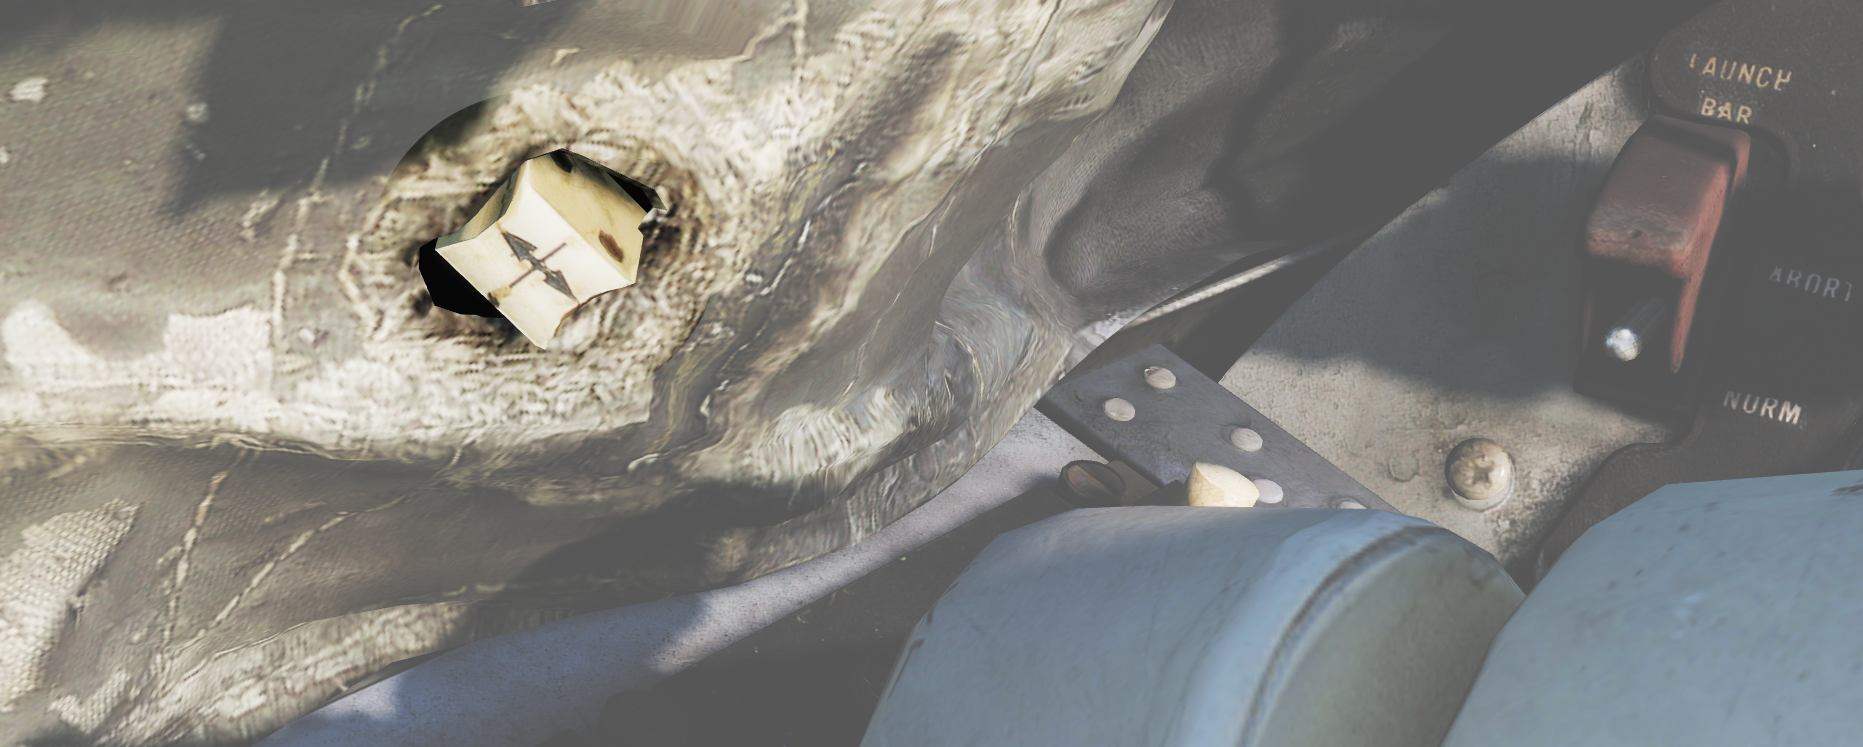
\includegraphics[width=0.8\textwidth]{target.png}
\end{figure}

用于在 HUD 中指定地面目标,也用于控制飞行员 ACM 雷达模式,但 PLM(飞行员锁定模式)模式除外。开关可以上下拨动,也可以向前拨动至目标指定档位。

空对地模式中,上/下拨动开关来移动指示符,向前拨动开关来指定目标。在其他模式中,上/下拨动开关分别选择 VSL HI(垂直扫描锁定 - 高目标)和VSL LO(垂直扫描锁定 - 低目标)ACM模式,而向前拨动开关选择 PAL 模式。

\subsubsection{进气道斜板 / 油门控制面板}

\begin{figure}[h]
  \center
  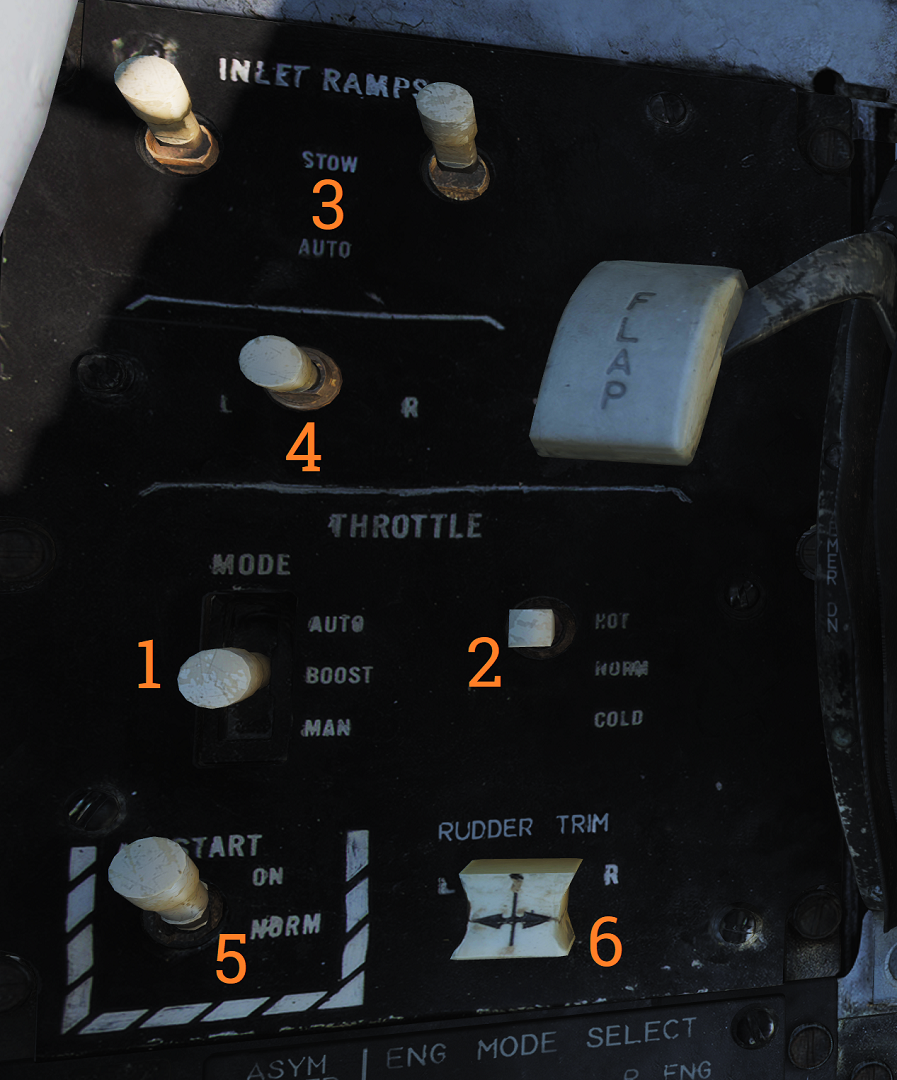
\includegraphics[width=0.8\textwidth]{inlet.png}
\end{figure}

这个面板用于控制多个发动机系统、油门设置以及方向舵配平。

\begin{enumerate}
  \item THROTTLE MODE 开关:油门模式开关,用于选择油门工作模式。
  \begin{itemize}
    \item AUTO:自动模式。
    \item BOOST:助力模式。
    \item MAN:手动模式。
  \end{itemize}
  \item THROTTLE TEMP 开关:油门温控开关,用于选择油门计算机增益。
  \begin{itemize}
    \item HOT:增大标准油门计算机增益。
    \item NORM:使用标准油门计算机增益。
    \item COLD:减小标准油门计算机增益。
  \end{itemize}
  \item INLET RAMPS 开关:进气道斜板开关,用于选择左右发动机各自的进气道斜板工作模式。
  \begin{itemize}
    \item STOW:收起。
    \item ATUO:自动模式。
  \end{itemize}
  \item ENG CRANK 开关:发动机起动开关,用于起动左发动机或右发动机。
  \item BACK UP IGNITION 开关:备用点火开关,用于开启或关闭备用点火。
  \item RUDDER TRIM 开关:方向舵配平开关,用于调整方向舵配平。
\end{enumerate}

\subsubsection{油门握把}

\begin{figure}[h]
  \center
  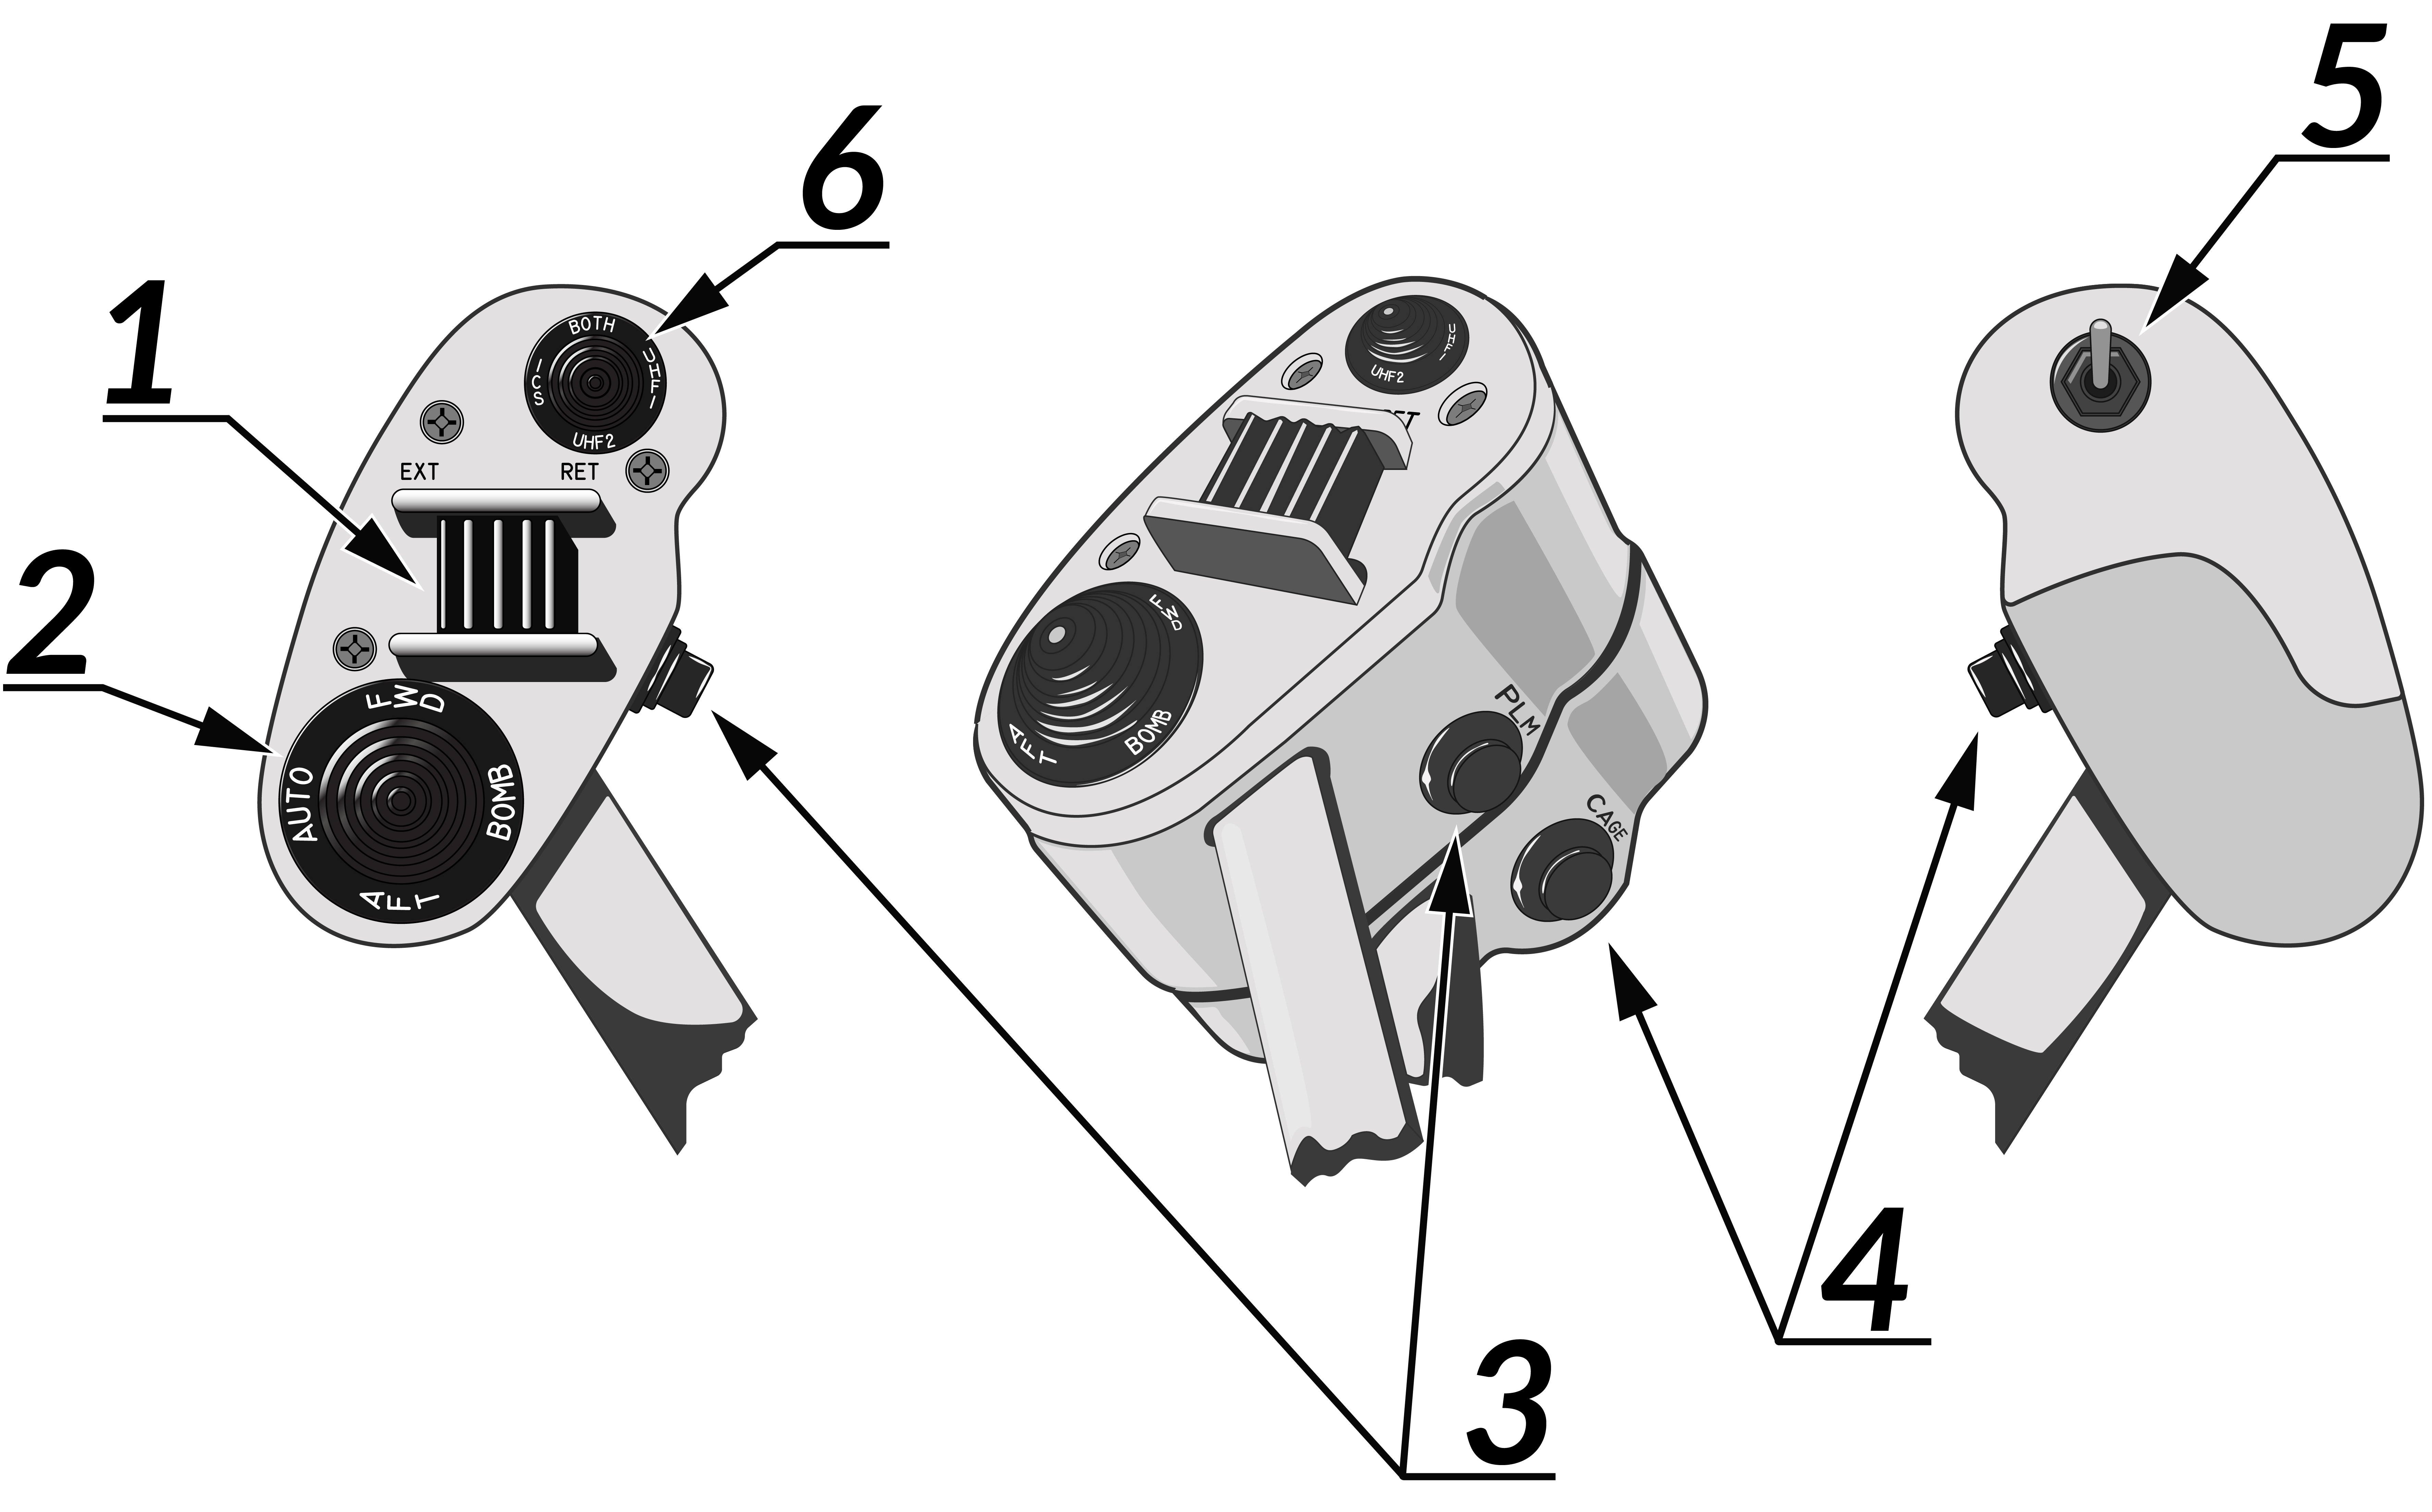
\includegraphics[width=0.8\textwidth]{throttle.png}
\end{figure}
油门握把上包括了各种飞行控制和 HOTAS(手不离杆)功能。

\begin{enumerate}
  \item 减速板开关:用于控制减速板展开和收起。
  \begin{itemize}
    \item EXT:释放开关后,回到中间位置。将开关保持在 EXT 档位会逐渐展开减速板。开关回中后,减速板仍会保持在当前位置。
    \item RET:将开关拨至该位置来收起减速板。
  \end{itemize}
  \item 机翼后掠控制开关:这个开关用于控制机翼后掠功能。手动模式下选择的后掠位置只能比 CADC 设置的位置靠后(后掠角度不能小于 CADC 指令后掠角)。
  \begin{itemize}
    \item AUTO:机翼后掠位置由 CADC(中央大气数据计算机) 自动设置。
    \item FWD:手动向前调节机翼后掠位置。
    \item AFT:手动向后调节机翼后掠位置。
    \item BOMB:如果机翼后掠角度小于55°,则将机翼后掠至55°位置。如果 CADC 设置的后掠位置超过55°,则将后掠位置调整至 CADC 设定的角度。
  \end{itemize}
  \item PLM按钮:飞行员锁定模式按钮,用于选择 AWG-9 的 ACM 飞行员锁定模式。也用于在 ACL(自动助降)过程中解除自动驾驶。
  \item CAGE/SEAM按钮:用于控制 AIM-9 导弹 CAGE(导引头解锁)/ SEAM(“响尾蛇”扩展搜索模式) 并启用 AIM-9 导引头锁定。如果启用了 APC(进近推力补偿器),则用于解除 APC。
  \item 机外照明开关:用于控制机外照明。OFF 档位会关闭所有机外照明,并增加进近指示灯亮起度。ON 档位会开启所有机外照明,并减小进近指示灯亮起度。
  \item ICS按键通话开关:通过这个开关,飞行员可以选择在单波道或双波道 V/UHF 下通话,或与 RIO 对讲。
  \begin{itemize}
    \item ICS:与RIO通话。
    \item BOTH:同时在 UHF 1 和 V/UHF 2 频率下通话。
    \item UHF1:在 UHF 1 频率下通话。
    \item UHF2:在 V/UHF 2 频率下通话。
  \end{itemize}
\end{enumerate}

\subsubsection{油门弧座}

\begin{figure}[h]
  \center
  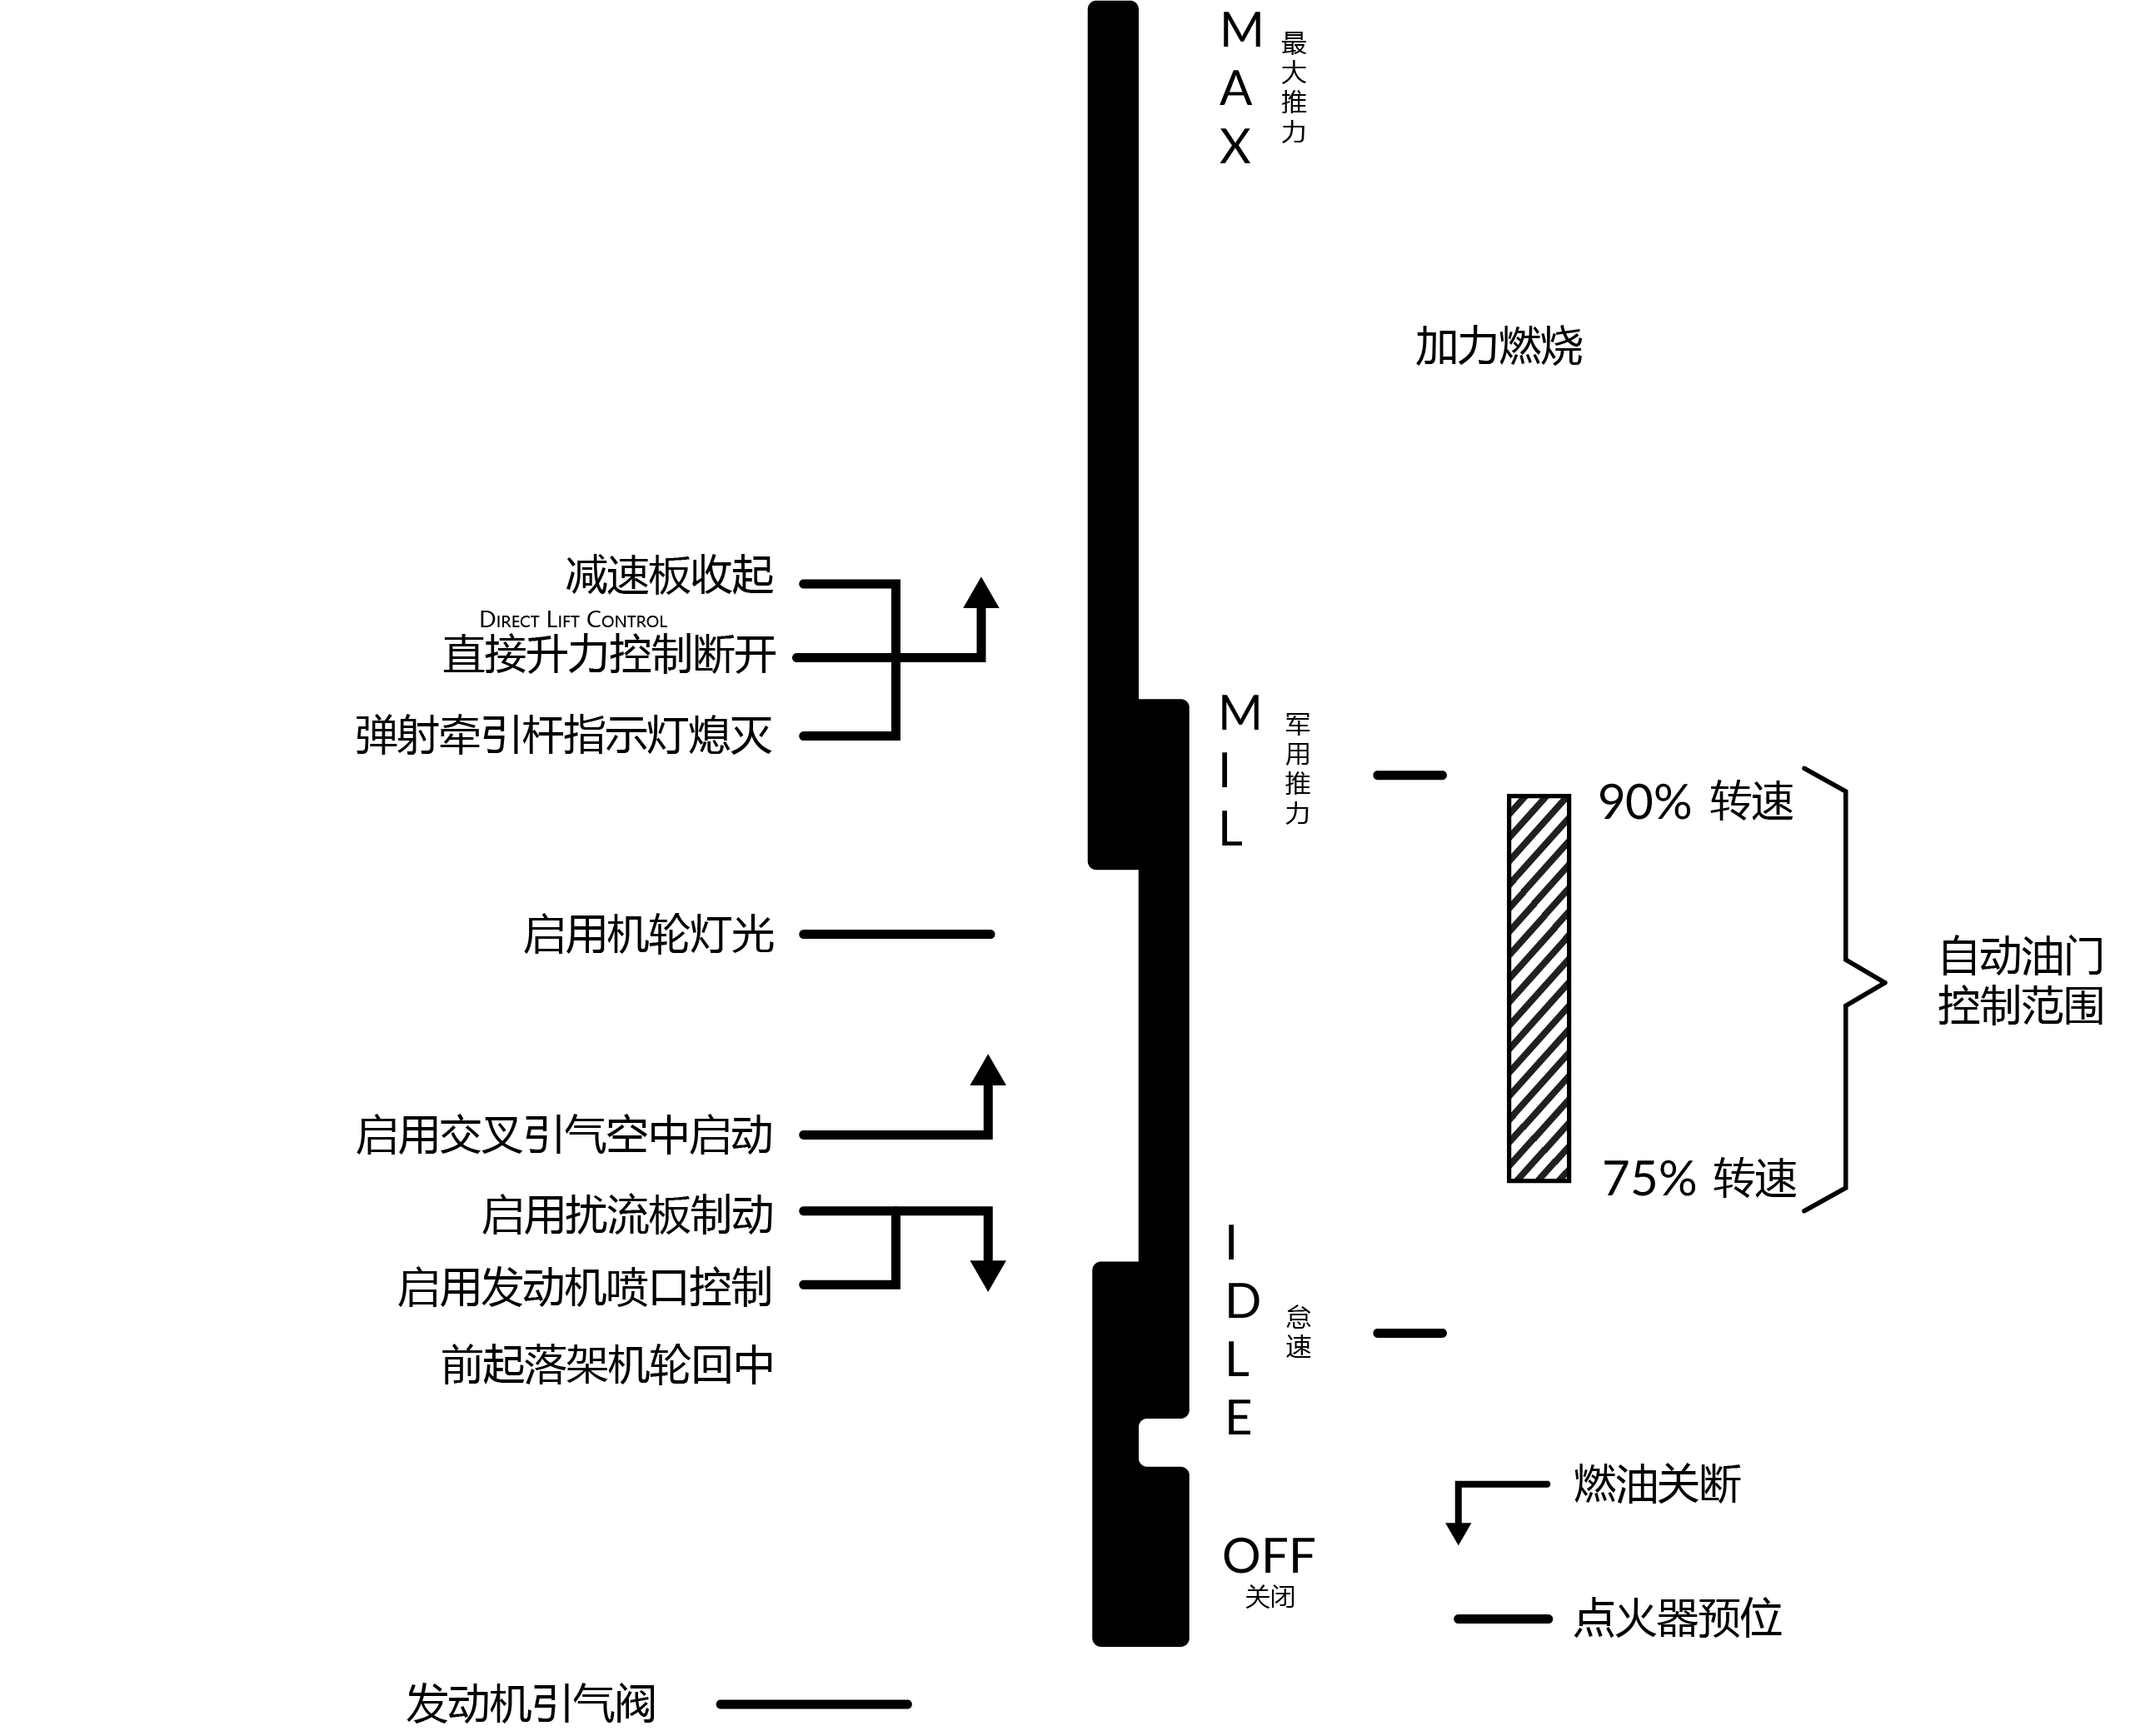
\includegraphics[width=0.8\textwidth]{throttles-schem.png}
\end{figure}
油门弧座主要组成部分包括:两个发动机油门控制握把、襟翼控制杆和应急机翼后掠手柄,另外也包括油门握把上用于控制 HOTAS 系统的按钮和开关。油门行程中的 OFF(关闭)、IDLE(慢车)和 MIL(军用推力)位置都有限动卡。

将油门从 OFF 位置推到 IDLE 位置会激活点火器并关闭发动机断油装置。油门握把内并未安装弹簧机构,横向推动油门时,握把不会被弹回原位,因此飞行员在弹射起飞时,可以将油门握把置于 MIL(军用推力)档,而不用担心油门位置意外变动,从而导致发动机转速降低。油门弧座左侧,襟翼控制杆的下方装有一个油门阻尼调节杆,用于选择所需的油门移动阻尼。

襟翼控制杆的无级行程的最前段和最后段分别有两个应急档位,一个是应急收上,一个是应急放下。两个应急档位都有限动卡,襟翼控制杆移动至限动卡位置时,需向外推动才能继续移动至应急档位。应急收上档位会强行收起襟翼,超控正常襟翼控制逻辑。应急放下档位无功能。

手动/应急机翼后掠手柄上方有一个保护盖,且手柄通常处于推入并收起的状态。握住手柄顶部,抽出手柄来进行手动机翼后掠控制。请查阅应急模式来获得更多相关信息。

\subsubsection{手动液压泵}

手动液压泵位于油门弧座的内侧,靠近飞行员左腿的位置。液压系统故障时,飞行员通过手动向机轮刹车蓄压器充压来进行制动操作(当起落架手柄处于放下档位时)或伸出受油管。

\subsection{左侧垂直控制台}
\subsubsection{燃油管理面板}

\begin{figure}[h]
  \center
  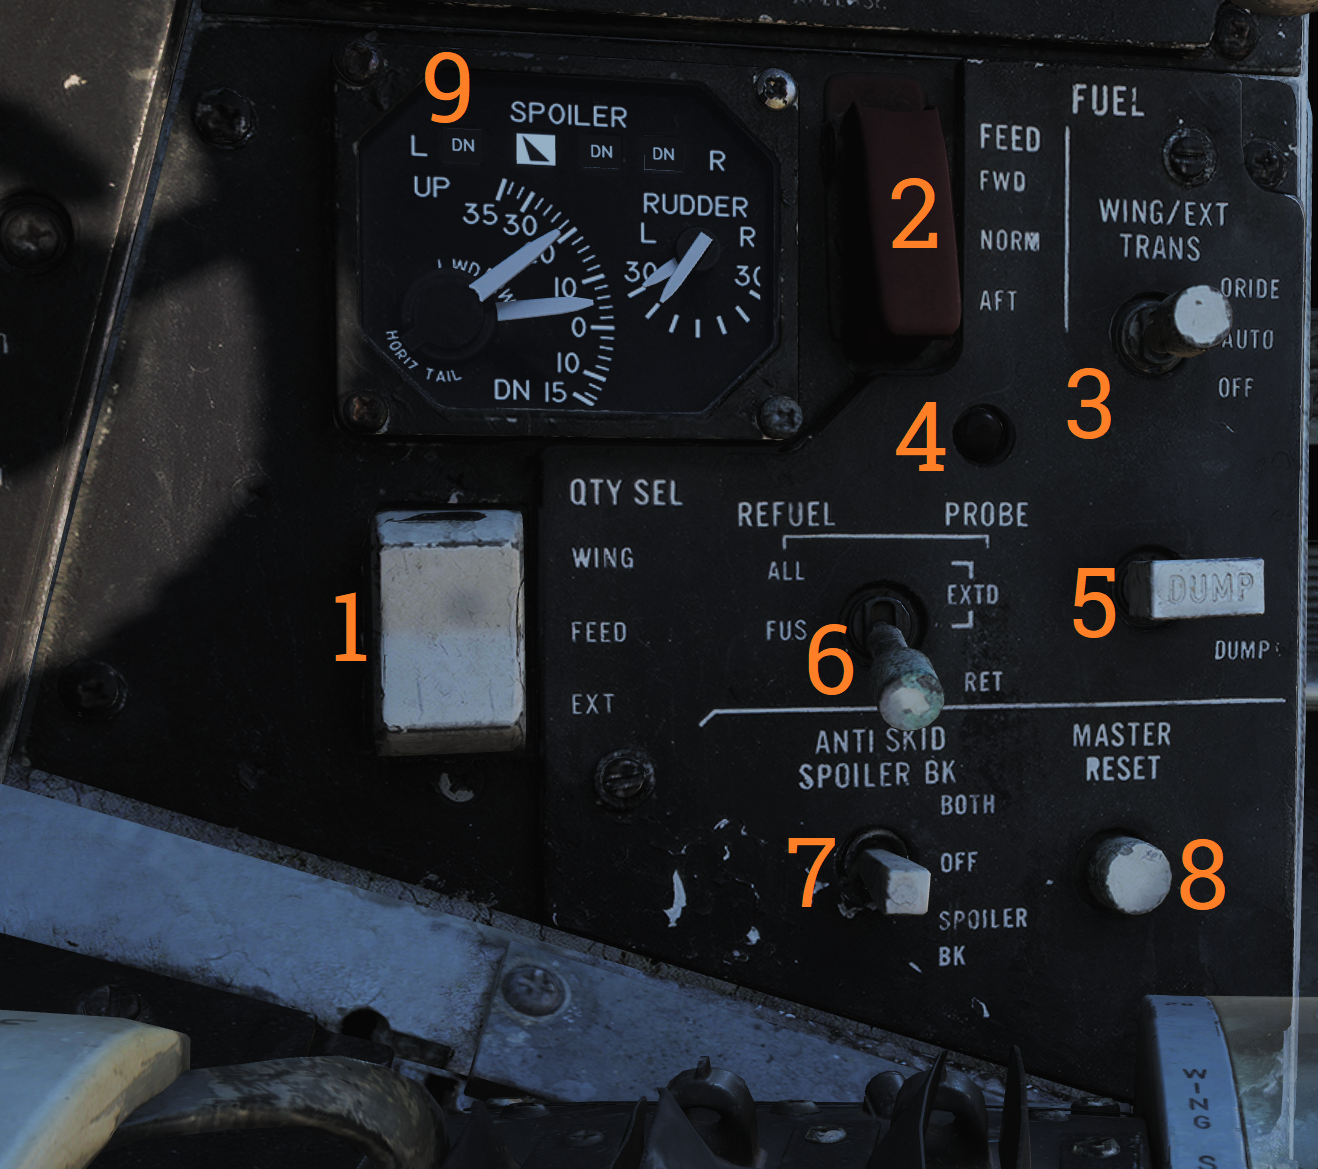
\includegraphics[width=0.8\textwidth]{fuel.png}
\end{figure}
这个面板用于控制诸多燃油相关系统、CADC 复位和防滑系统。

\begin{enumerate}
  \item QTY SEL 选择开关:燃油量选择开关,这个滑动弹簧开关用于选择燃油量条状指示器上显示哪个油箱中的燃油量。松开开关后,开关会弹回 FEED 档位。
  \begin{itemize}
    \item FEED:供油油箱,显示供油油箱和机身油箱中的燃油量。
    \item WING:机翼油箱,显示各个机翼油箱中的燃油量。
    \item EXT:副油箱,显示副油箱中的燃油量。
  \end{itemize}
  \item FEED 开关:供油油箱选择开关,用于选择为发动机供油的油箱。保护盖关闭时,开关被锁定在 NORM 档位。
  \item WING/EXT TRANS 开关:机翼/副油箱转移开关,用于控制机翼油箱和副油箱中的燃油转移。
  \begin{itemize}
    \item ORIDE:超控。
    \item AUTO:一般使用的档位。
    \item OFF:停止机翼和副油箱的燃油传输。
  \end{itemize}
  \item 受油管指示灯:当受油管未完全伸出,或未完全收起时,指示灯便会亮起。
  \item DUMP 开关:放油开关,用于开启或停止放油。减速板收起,机轮不负重且加力燃烧关闭时飞机可以进行放油操作。
  \item REFUEL PROBE 开关:受油管开关,用于伸出或收起受油管。
  \begin{itemize}
    \item ALL EXTD:受油管移动至完全伸出位置,允许对所有(ALL)油箱受油。同时也会将机翼/副油箱转移开关(WING/EXT TRANS)复位回 AUTO 档位。
    \item FUS EXTD:受油管移动至完全伸出位置,只允许对机身(FUS)油箱受油。
    \item RET:收起受油管。
  \end{itemize}
  \item ANTI SKID SPOILER BK 开关:防滑和扰流板制动开关,用于选择和控制防滑系统和扰流板制动系统。
  \begin{itemize}
    \item BOTH:机轮负重时,启用防滑系统和扰流板制动系统。
    \item OFF:关闭防滑系统和扰流板制动系统。
    \item SPOILER BK:扰流板制动,机轮负重时,启用扰流板制动功能。
  \end{itemize}
  \item MASTER RESET 按钮:CADC 主复位按钮,用于复位 CADC 故障检测系统及相关故障显示。
  \item 操纵面位置指示器:显示操纵面位置。详见下文。
\end{enumerate}

\subsubsection{操纵面位置指示器}

\begin{figure}[h]
  \center
  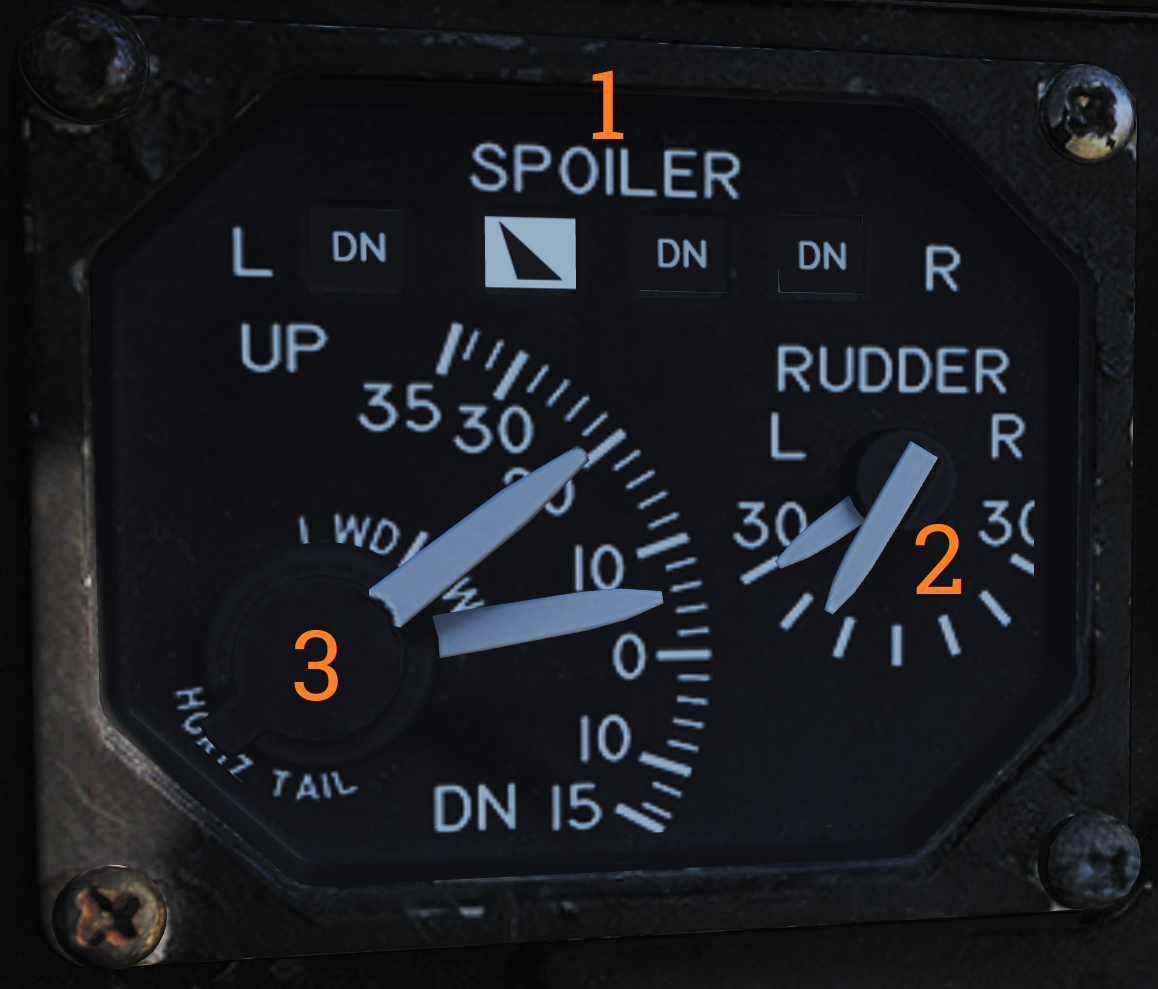
\includegraphics[width=0.8\textwidth]{control.png}
\end{figure}
操纵面位置指示器是用于指示各个飞行操纵面位置的仪表。

\begin{enumerate}
  \item SPOILER 指示器:扰流板位置指示器。
  \begin{itemize}
    \item DN:扰流板收起,与机翼齐平。
    \item 向上箭头:扰流板伸出。
    \item 向下箭头:扰流板放下至机翼表面下方。
  \end{itemize}
  \item RUDDER 指示器:方向舵位置指示器,标注的“L”和“R”分别指示了左方向舵和右方向舵的位置。
  \item HORIZ TAIL 指示器:水平安定面位置指示器,标注的“L”和“R”分别显示了左水平安定面和右水平安定面的位置。
\end{enumerate}

\subsubsection{弹射杆中止面板}

\begin{figure}[h]
  \center
  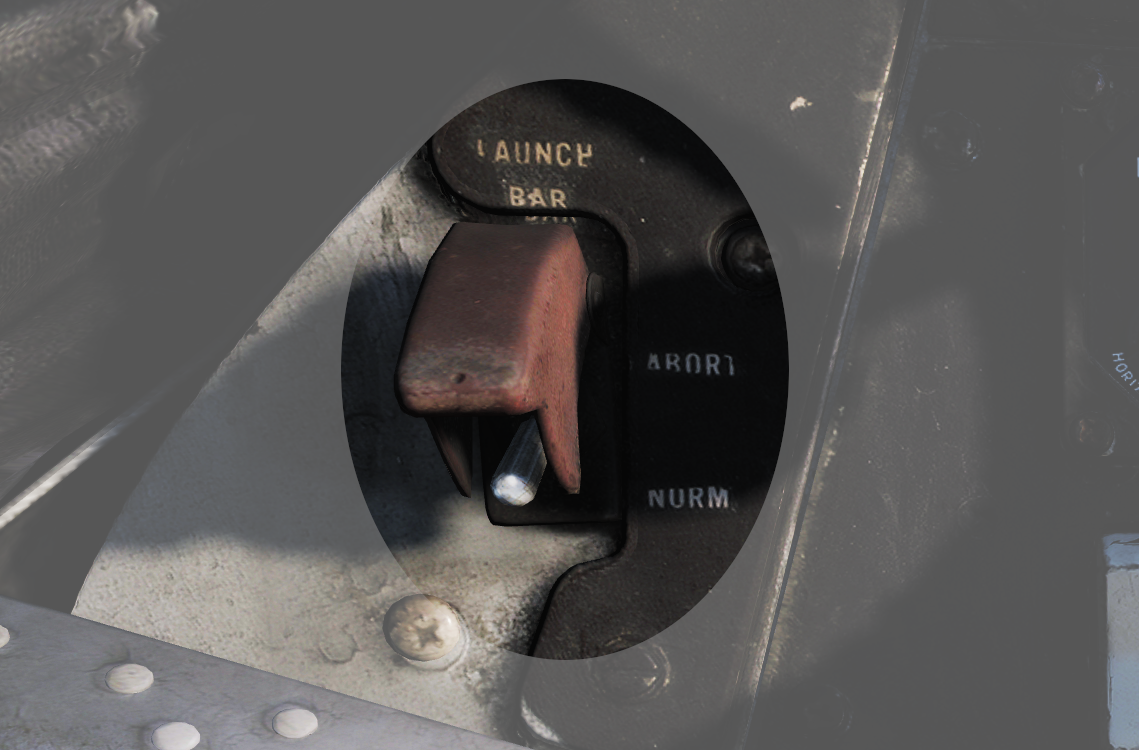
\includegraphics[width=0.8\textwidth]{launch-abort.png}
\end{figure}
弹射杆选择开关,将弹簧开关保持在 ABORT 档位时,弹射杆升起,终止弹射。松开开关后,开关弹回 NORM (正常)档位,这也是弹射杆选择开关的标准位置。目前,这个开关在 DCS 中没有实际作用。

\subsubsection{起落架控制面板}

\begin{figure}[h]
  \center
  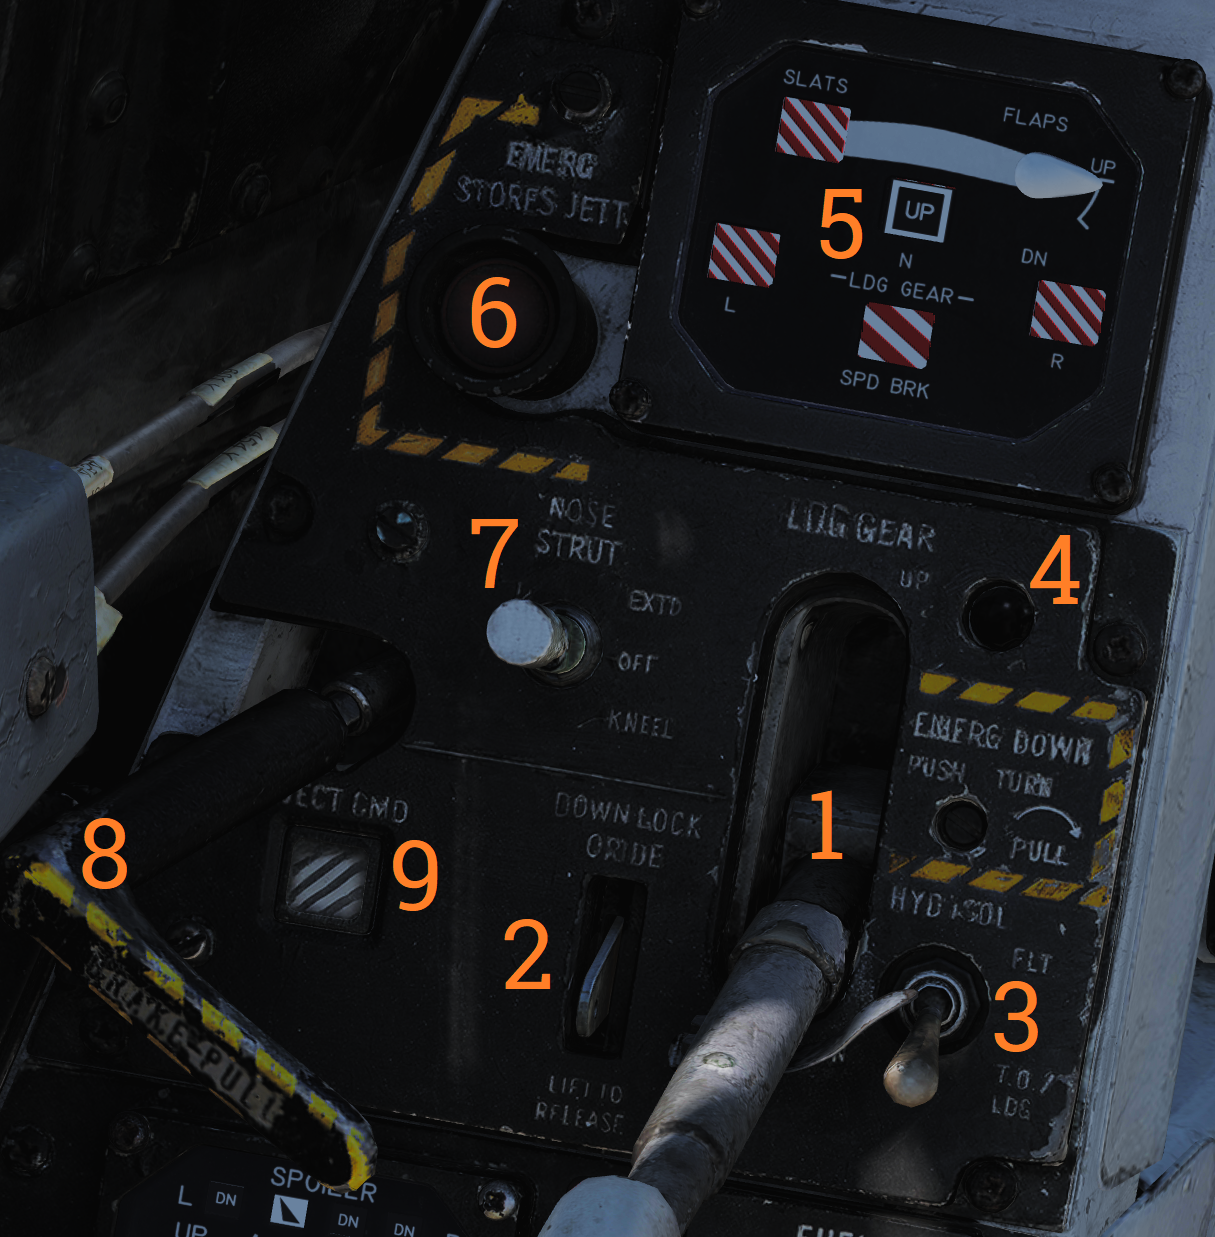
\includegraphics[width=0.8\textwidth]{gear.png}
\end{figure}
这个面板用于控制主起落架和应急挂载抛离。

\begin{enumerate}
  \item LDG GEAR 手柄:起落架控制手柄,用于选择起落架的 UP(收上)或 DOWN(放下)位置。紧急情况下(液压失效等),将手柄置于向下位置,并将手柄推入,顺时针旋转手柄顶端然后抽出。这会释放储存的压缩氮气,使起落架紧急放下。
  \item DOWN LOCK ORIDE 杆:起落架放下锁定超控杆,被电磁铁移动至向下位置时指示机轮负重。可以升起至向上位置来超控(起落架手柄锁定在 DOWN 位置)。DCS 中无功能。
  \item HYD ISOL 开关:起落架液压隔离开关,用于将起落架、前轮转向和机轮刹车的液压控制隔离出联合液压系统。起落架手柄处于放下位置时,隔离开关由起落架手柄自动移动至 T.O. / LDG 档位。
  \begin{itemize}
    \item FLT:空中飞行时,隔离上述系统中的液压控制。
    \item T.O. / LDG:起飞/降落,接通上述系统的液压控制,允许它们正常工作。
  \end{itemize}
  \item 起落架位置转移指示灯:起落架实际位置与起落架控制手柄位置不符时,指示灯会亮起。
  \item 机轮-襟翼位置指示器:详见下文。
  \item EMERG STORES 按钮:应急挂载抛离按钮,按下时会亮起,表示激活应急抛离。
  \item NOSE STRUT 开关:前轮支柱开关,这个弹簧开关用于控制前起落架支柱伸缩。
  \begin{itemize}
    \item EXTD:伸展前起落架支柱,升起并锁定弹射杆。
    \item OFF:关闭前起落架支柱运动,松开开关时,开关弹回该位置。
    \item KNEEL:减小前起落架支柱系统中的液压压强,使支柱收缩,从而降低机头的高度,同时解锁弹射杆。
  \end{itemize}
  \item BRAKE-PULL 手柄:制动-抽出手柄,用于控制停放刹车,抽出手柄来启动停放刹车,推入手柄释放机轮刹车。
  \item EJECT CMD 指示器:弹射指令指示器,指示后座驾驶舱的弹射系统的模式。
  \begin{itemize}
    \item PILOT:飞行员弹射时弹射所有机组乘员,RIO 弹射时只弹射自己。
    \item MCO:飞行员或 RIO 弹射时,另一名机组乘员也会被弹射。
  \end{itemize}
\end{enumerate}

\subsubsection{机轮-襟翼位置指示器}

\begin{figure}[h]
  \center
  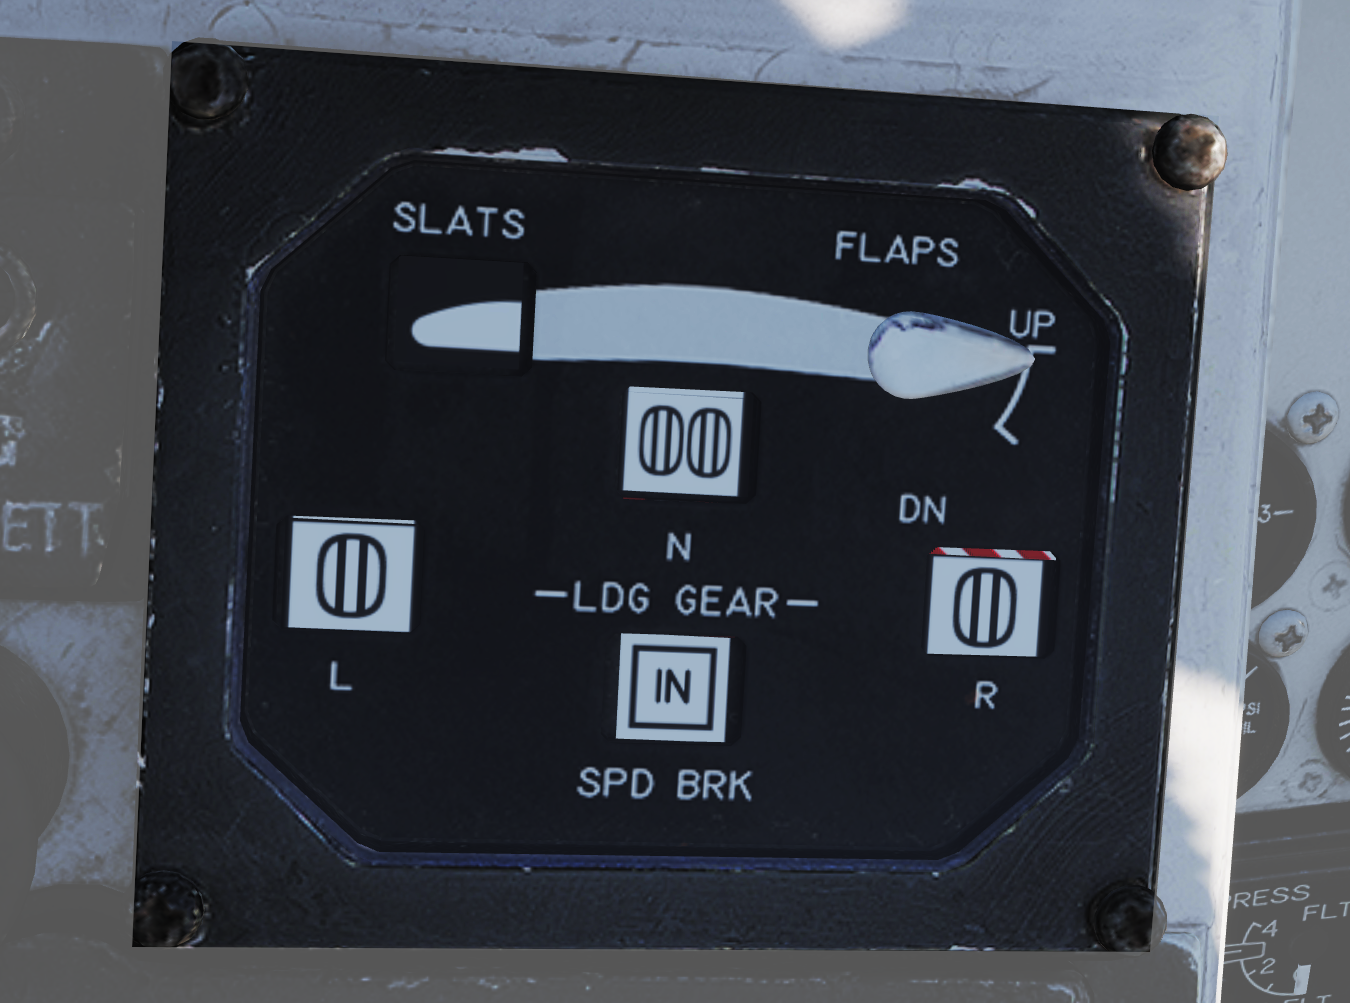
\includegraphics[width=0.8\textwidth]{wheels-flaps.png}
\end{figure}
指示襟翼和前缘缝翼、减速板和起落架的位置。前缘缝翼的位置指示标识如下:
\begin{itemize}
  \item 
\includegraphics[width=1.0cm]{off.png}:电源切断,或前缘机动缝翼张开。
  \item 
\includegraphics[width=1.0cm]{slats-ext.png}:前缘缝翼放下。
  \item 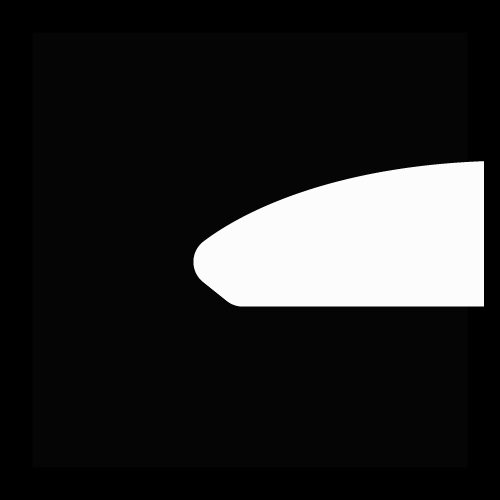
\includegraphics[width=1.0cm]{slats-ret.png}:前缘缝翼收上。
\end{itemize}

\subsection{左膝仪表板}

\subsection{左仪表板}

\subsection{风挡左边框}

\subsection{风挡右边框}

\subsection{右仪表板}

\subsection{右膝仪表板}

\subsection{右侧垂直控制台}

\subsection{右侧控制台}

\subsection{座舱盖控制手柄}

\section{雷达拦截官驾驶舱}

\subsection{左侧控制台}

\subsection{左侧垂直控制台}

\subsection{左仪表板}

\subsection{中央仪表板}

\subsection{中央控制台}


\subsection{左右脚部空间}

\subsection{右仪表板}

\subsection{右膝仪表板}

\subsection{右侧垂直控制台}

\subsection{右侧控制台}

\subsection{座舱盖控制手柄}

% \chapter{图表公式例子}
% \label{cha:chapter02}

% \section{其它例子}
% \label{sec:other}

% 在第~\ref{cha:intro} 章中我们学习了贝叶斯公式~(\ref{equ:chap1:bayes}),这里我们复
% 习一下:
% \begin{equation}
% \label{equ:chap2:bayes}
% p(y|\vx) = \frac{p(\vx,y)}{p(\vx)}=
% \frac{p(\vx|y)p(y)}{p(\vx)}
% \end{equation}

% \subsection{绘图}
% \label{sec:draw}

% 本模板不再预先装载任何绘图包(如 \pkg{pstricks,pgf} 等),完全由用户来决定。
% 个人觉得 \pkg{pgf} 不错,不依赖于 Postscript。此外还有很多针对 \LaTeX{} 的
%  GUI 作图工具,如 XFig(jFig), WinFig, Tpx, Ipe, Dia, Inkscape, LaTeXPiX,
% jPicEdt, jaxdraw 等等。

% \subsection{插图}
% \label{sec:graphs}

% 强烈推荐《\LaTeXe{} 插图指南》!关于子图形的使用细节请参看 \pkg{subcaption} 宏包的说明文档。

% \subsubsection{一个图形}
% \label{sec:onefig}
% 一般图形都是处在浮动环境中。之所以称为浮动是指最终排版效果图形的位置不一定与源文
% 件中的位置对应\footnote{This is not a bug, but a feature of \LaTeX!},这也是刚使
% 用 \LaTeX{} 同学可能遇到的问题。如果要强制固定浮动图形的位置,请使用 \pkg{float} 宏包,
% 它提供了 \texttt{[H]} 参数,比如图~\ref{fig:xfig1}。
% \begin{figure}[H] % use float package if you want it here
%   \centering
%   
\includegraphics{thu-whole-logo.pdf}
%   \caption{利用 Xfig 制图}
%   \label{fig:xfig1}
% \end{figure}

% 大学之道,在明明德,在亲民,在止于至善。知止而后有定;定而后能静;静而后能安;安
% 而后能虑;虑而后能得。物有本末,事有终始。知所先后,则近道矣。古之欲明明德于天
% 下者,先治其国;欲治其国者,先齐其家;欲齐其家者,先修其身;欲修其身者,先正其心;
% 欲正其心者,先诚其意;欲诚其意者,先致其知;致知在格物。物格而后知至;知至而后
% 意诚;意诚而后心正;心正而后身 修;身修而后家齐;家齐而后国治;国治而后天下
% 平。自天子以至于庶人,壹是皆以修身为本。其本乱而未治者 否矣。其所厚者薄,而其所
% 薄者厚,未之有也!

% \hfill —— 《大学》


% \subsubsection{多个图形}
% \label{sec:multifig}

% 如果多个图形相互独立,并不共用一个图形计数器,那么
% 用 \texttt{minipage} 或者\texttt{parbox} 就可以。否则,请参看
% 图~\ref{fig:big1-subcaptionbox},它包含两个小图,分别是图~\ref{fig:subfig1}和
% 图~\ref{fig:subfig2}。推荐使用 \cs{subcaptionbox},因为可以像
% 图~\ref{fig:big1-subcaptionbox} 那样对齐子图的标题,也可以使用 \pkg{subcaption}
% 宏包的 \cs{subcaption}(放在 minipage中,用法同\cs{caption})或
% 是 \pkg{subfigure} 、\pkg{subtable}环境,像图~\ref{fig:big1-subfigure},不要再
% 用 \cs{subfloat}、\cs{subfigure} 和 \cs{subtable}。

% \begin{figure}[h]
%   \centering%
%   \subcaptionbox{第一个小图形\label{fig:subfig1}}[3cm] %标题的长度,超过则会换行,如下一个小图。
%     {
\includegraphics[height=3cm]{thu-fig-logo.pdf}}%
%   \hspace{4em}%
%   \subcaptionbox{第二个小图形,注意这个图略矮些。如果标题很长的话,它会自动换行\label{fig:subfig2}}
%       {
\includegraphics[height=2cm]{thu-text-logo.pdf}}
%   \caption{包含子图形的大图形(subcaptionbox示例)}
%   \label{fig:big1-subcaptionbox}
% \end{figure}
% \begin{figure}[h]
%   \centering%
%   \begin{subfigure}{3cm}
%     
\includegraphics[height=3cm]{thu-fig-logo.pdf}
%     \caption{第一个小图形}
%   \end{subfigure}%
%   \hspace{4em}%
%   \begin{subfigure}{0.5\textwidth}
%     
\includegraphics[height=2cm]{thu-text-logo.pdf}
%     \caption{第二个小图形,注意这个图略矮些。subfigure中同一行的子图在顶端对齐。}
%   \end{subfigure}
%   \caption{包含子图形的大图形(subfigure示例)}
%   \label{fig:big1-subfigure}
% \end{figure}

% 古之学者必有师。师者,所以传道受业解惑也。人非生而知之者,孰能无惑?惑而不从师,
% 其为惑也,终不解矣。生乎吾前,其闻道也固先乎吾,吾从而师之;生乎吾後,其闻道也亦
% 先乎吾,吾从而师之。吾师道也,夫庸知其年之先後生於吾乎!是故无贵无贱无长无少,道
% 之所存,师之所存也。

% 嗟乎!师道之不传也久矣,欲人之无惑也难矣。古之圣人,其出人也远矣,犹且从师而问焉;
% 今之众人,其下圣人也亦远矣,而耻学於师。是故圣益圣,愚益愚。圣人之所以为圣,愚
% 人之所以为愚,其皆出於此乎?爱其子,择师而教之,於其身也,则耻师焉,惑焉。彼童子
% 之师,授之书而习其句读者,非吾所谓传其道、解其惑者也。句读之不知,惑之不解,或师
% 焉,或不焉,小学而大遗,吾未见其明也。巫医、乐师、百工之人不耻相师,  士大夫之族
% 曰“师”曰“弟子”之云者,则群聚而笑之。问之,则曰:彼与彼年相若也,道相似也,位
% 卑则足羞,官盛则近谀。呜呼!师道之不复,可知矣。巫医、乐师、百工之人。吾子不齿,
% 今其智乃反不能及,其可怪也欤!圣人无常师。孔子师郯子、苌子、师襄、老聃。郯子之徒,
% 其贤不及孔子。孔子曰:“三人行,必有我师。”是故弟子不必不如师,师不必贤於弟子。
% 闻道有先後,术业有专攻,如是而已。

% 如果要把编号的两个图形并排,那么小页就非常有用了:
% \begin{figure}
% \begin{minipage}{0.48\textwidth}
%   \centering
%   
\includegraphics[height=2cm]{thu-whole-logo.pdf}
%   \caption{并排第一个图}
%   \label{fig:parallel1}
% \end{minipage}\hfill
% \begin{minipage}{0.48\textwidth}
%   \centering
%   
\includegraphics[height=2cm]{thu-whole-logo.pdf}
%   \caption{并排第二个图}
%   \label{fig:parallel2}
% \end{minipage}
% \end{figure}

% 李氏子蟠,年十七,好古文、六艺,经传皆通习之,不拘於时,学於余。余嘉其能行古
% 道,作师说以贻之。

% \hfill —— 韩愈(唐)
